\documentclass{article}

\usepackage{arxiv}

\usepackage[utf8]{inputenc} % allow utf-8 input
\usepackage[T1]{fontenc}    % use 8-bit T1 fonts
\usepackage{lmodern}        % https://github.com/rstudio/rticles/issues/343
\usepackage{hyperref}       % hyperlinks
\usepackage{url}            % simple URL typesetting
\usepackage{booktabs}       % professional-quality tables
\usepackage{amsfonts}       % blackboard math symbols
\usepackage{nicefrac}       % compact symbols for 1/2, etc.
\usepackage{microtype}      % microtypography
\usepackage{graphicx}

\title{Ancestral state reconstruction of phenotypic characters}

\author{
    Liam J. Revell
   \\
    Department of Biology \\
    University of Massachusetts Boston \\
  Boston, MA 02125 \\
  \texttt{\href{mailto:liam.revell@umb.edu}{\nolinkurl{liam.revell@umb.edu}}} \\
  }


% tightlist command for lists without linebreak
\providecommand{\tightlist}{%
  \setlength{\itemsep}{0pt}\setlength{\parskip}{0pt}}

% From pandoc table feature
\usepackage{longtable,booktabs,array}
\usepackage{calc} % for calculating minipage widths
% Correct order of tables after \paragraph or \subparagraph
\usepackage{etoolbox}
\makeatletter
\patchcmd\longtable{\par}{\if@noskipsec\mbox{}\fi\par}{}{}
\makeatother
% Allow footnotes in longtable head/foot
\IfFileExists{footnotehyper.sty}{\usepackage{footnotehyper}}{\usepackage{footnote}}
\makesavenoteenv{longtable}

% Pandoc citation processing
%From Pandoc 3.1.8
% definitions for citeproc citations
\NewDocumentCommand\citeproctext{}{}
\NewDocumentCommand\citeproc{mm}{%
  \begingroup\def\citeproctext{#2}\cite{#1}\endgroup}
\makeatletter
 % allow citations to break across lines
 \let\@cite@ofmt\@firstofone
 % avoid brackets around text for \cite:
 \def\@biblabel#1{}
 \def\@cite#1#2{{#1\if@tempswa , #2\fi}}
\makeatother
\newlength{\cslhangindent}
\setlength{\cslhangindent}{1.5em}
\newlength{\csllabelwidth}
\setlength{\csllabelwidth}{3em}
\newenvironment{CSLReferences}[2] % #1 hanging-indent, #2 entry-spacing
 {\begin{list}{}{%
  \setlength{\itemindent}{0pt}
  \setlength{\leftmargin}{0pt}
  \setlength{\parsep}{0pt}
  % turn on hanging indent if param 1 is 1
  \ifodd #1
   \setlength{\leftmargin}{\cslhangindent}
   \setlength{\itemindent}{-1\cslhangindent}
  \fi
  % set entry spacing
  \setlength{\itemsep}{#2\baselineskip}}}
 {\end{list}}
\usepackage{calc}
\newcommand{\CSLBlock}[1]{#1\hfill\break}
\newcommand{\CSLLeftMargin}[1]{\parbox[t]{\csllabelwidth}{#1}}
\newcommand{\CSLRightInline}[1]{\parbox[t]{\linewidth - \csllabelwidth}{#1}\break}
\newcommand{\CSLIndent}[1]{\hspace{\cslhangindent}#1}

\usepackage{amsmath,mathtools,bm,nicematrix}

\begin{document}
\maketitle


\begin{abstract}
Ancestral state reconstruction is a phylogenetic comparative method that involves estimating the unknown trait values of hypothetical ancestral taxa at internal nodes of a phylogenetic tree. Ancestral state reconstruction has long been, and continues to remain, among the most popular analyses in phylogenetic comparative research. In this review, I illustrate the theory and practice of ancestral state reconstruction for both discretely and continuously-valued phenotypic traits. For discrete characters, I focus on the M\emph{k} model and describe the distinction between marginal and joint reconstruction, as well as between local vs.~global estimation. For continuous traits, I describe ancestral state reconstruction under a model of Brownian motion evolution. I highlight several use cases of ancestral state reconstruction \emph{via} a set of empirical examples, ranging from diel activity pattern in primates, to environmental tolerance in lizards. Finally, I discuss and explore the statistical properties of ancestral state estimation as well as its limitations. By illustrating ancestral reconstruction under the hidden-rates and threshold models (for discrete traits), and bounded Brownian motion (for continuous characters), I demonstrate the considerable sensitivity of ancestral reconstruction to model misspecification. Although ancestral state reconstruction is virtually certain to retain its popularity into the future, I conclude by recommending considerable caution and circumspection in the use and interpretation of ancestral reconstruction in empirical evolutionary research.
\end{abstract}


\section{Introduction}\label{introduction}

Ancestral state reconstruction\footnote{Ancestral state reconstruction is also often referred to as \emph{ancestral character estimation}. These are the same thing, and I'll use the two terms interchangeably here.} is the general practice of estimating the value or values of a feature or attribute at the set of common ancestors of the operational taxa\footnote{Operational taxa are the named tips or leaves in a reconstructed phylogeny. In many studies using phylogenetic comparative methods operational taxa are nominal species, but they could also be subspecies, populations, cultural groups (in the case of language phylogenies), genera, or other units of study (e.g., Walker et al. 2012; Hall et al. 2018; Yaxley and Foley 2019; Li et al. 2022).} of a phylogenetic tree (Schluter et al. 1997; Yang 2006, 2014; Revell and Harmon 2022). Ancestral state reconstruction falls within the domain of phylogenetic comparative methods\footnote{For the purposes of this article, phylogenetic comparative methods are the set of methodologies that are used (typically) \emph{downstream} of phylogenetic inference to test hypotheses about evolution based on a tree, and often in combination with trait data for the terminal taxa of that tree.} (Pagel 1997; Nunn 2011; O'Meara 2012; Harmon 2019; Revell and Harmon 2022), and has long been relentlessly popular. The popularity of ancestral reconstruction is easy to comprehend. Evolutionary biologists are often inherently interested in the evolutionary past, and ancestral character estimation promises us a window towards that otherwise invisible history (Harvey and Pagel 1991; Revell and Harmon 2022).

Undertaking ancestral state reconstruction requires that we have a reconstructed tree\footnote{Or set of trees, e.g., from a bootstrapping analysis or Bayesian posterior sample.}\textsuperscript{,}\footnote{None of the methods of this article technically require that our input tree be ultrametric or time-calibrated. Normally, however, I recommend using an ultrametric or time-calibrated tree unless we have a formal, \emph{a priori} hypothesis that the rate of evolution of our trait is better predicted by non-ultrametric branch lengths -- for instance the branch lengths obtained from Maximum Likelihood phylogeny inference -- than by units of chronological time. The circumstances in which this is true are, I believe, quite rare.}, as well as observations of a phenotypic trait of interest from some or all of the terminal taxa of that tree (Harvey and Pagel 1991; Nunn 2011; Revell and Harmon 2022). Modern ancestral state reconstruction also requires that we have a model or hypothesized model for how our character trait evolved over the macroevolutionary time represented by our phylogeny.\footnote{At the risk of upsetting some enthusiasts, and apart from in this footnote, I will avoid discusing \emph{parsimony} as a method for ancestral state reconstruction here. Parsimony, better known as a technique of phylogeny inference, is a procedure whereby we seek to identify the set of ancestral states that will minimize the minimum number of evolutionary changes in our character that are required to explain the observed data pattern. This set of node values can then be characterized as the \emph{maximum parsimony} or \emph{most parsimonious} ancestral states. Even though this might seem sensible and will often provide very reasonable ancestral character estimates, parsimony leaves us with substantial difficulty in assessing the strength of evidence in support of this most parsimonious solution -- compared to, say, an alternative only slightly less parsimonious one -- and does not provide any firm criteria for averaging across any equally parsimonious sets of states. For this reason, and others, I have decided to focus on explicit, probabilistic procedures of ancestral state inference in this article.} Finally, we'll use a formal statistical inference procedure to obtain a set of estimates of our trait at some or all of the internal nodes of the tree.

In the sections below, I'll first offer some preliminaries on the goals of this article and on terminology. I'll then continue to describe the procedures for estimating ancestral phenotypes, first for discrete and then for continuously-valued traits, accompanying each section with a small number of empirical examples. Finally, I'll discuss some limitations of ancestral state estimation, focusing particularly on those arising from identifiable inadequacies of the assumed trait evolution model.

\section{Preliminaries}\label{preliminaries}

This article focuses on phylogenetic ancestral state reconstruction of discrete and continuously-valued phenotypic traits. A phylogenetic tree is a acyclic\footnote{Acyclic just means that the graph doesn't form loops or cycles.}, directed graph, typically used as a model to represent the historical relationships among species unified by common descent (Felsenstein 2004; Yang 2014; Revell and Harmon 2022). Phylogenies are also used to approximate other entities connected via a similar form of ancestor-descendant relationship, such as human cultural groups, viral sequences of an emerging infectious disease, or metastatic tumor cell lines in a cancer patient (e.g., Gray et al. 2009; Nunn 2011; Somarelli et al. 2017; Turakhia et al. 2020; Quinn et al. 2021).\footnote{For the most part, the methods of this article will be equally applicable to phylogenies employed in these other contexts.}

Phylogenies consist of three main components: nodes, branches, and tips (Yang 2006; Baum and Smith 2012; Revell and Harmon 2022). Nodes are hypothetical ancestral taxa located at the nexus point of two or more descendant branches. A branch (often referred to as an \emph{edge}, and I'll use the terms interchangeably here)\footnote{Branch is the term that predominates in the phylogenetic literature, whereas edge is used more commonly by biomathematicians and graph theoreticians.} is a connection between two different nodes: parent (i.e., ancestral) and daughter (i.e, descendant). Branches often have the property of length, which, in the type of tree used for ancestral state reconstruction, often represents elapsed time in some unit. Finally, a tip (often referred to as a \emph{leaf}, and I'll sometimes use that term here) is an external node of the tree, not connected to any descendant nodes, that is used to represent a species or other operational taxon of the phylogeny. Once again, in the type of phylogenetic tree used for ancestral state reconstruction, tips most often have as an attribute a label, indicating to which taxon they correspond (Felsenstein 2004; Baum and Smith 2012).

Though ancestral state reconstruction can also be undertaken for nucleotide sequence or other molecular characters (e.g., Yang 2014), in this article I'll focus on ancestral state reconstruction of phenotypic traits (Schluter et al. 1997; Nunn 2011; Revell and Harmon 2022). A phenotypic trait is an observable attribute -- be it physical, morphological, behavioral, ecological, physiological, cellular, etc. -- of the operational taxa of the tree. In the field of phylogenetic comparative biology, we conventionally subdivide phenotypic traits into two general categories (whilst realizing that some traits may not fall neatly into either): discrete and continuous (Pagel 1997; Felsenstein 2004; Revell and Harmon 2022; Revell 2024).

Discrete characters are phenotypic attributes that can only assume one of fixed and finite set of values (Revell and Harmon 2022). These might range from a discretely-categorized ecological trait (e.g., marine vs.~freshwater habitat use in fishes, Betancur‐R. et al. 2015), to a counted meristic character (e.g., pre-caudal vertebra number in primates, Spear et al. 2023), to a behavioral specialization (e.g., diel activity pattern in vertebrates, Anderson and Wiens 2017), to a categorical physical attribute (e.g., carotenoid-pigmented feathers in birds, Thomas et al. 2014).

Continuous characters, on the other hand, are phenotypic traits that can assume any of an infinite number of values on a real number scale (Revell and Harmon 2022). Continuous characters needn't be \emph{unbounded} -- for example, a continuous character is often bounded on the lower end by the value of zero. Nonetheless, unbounded evolution is a frequent assumption of continuous character models in phylogenetic comparative analysis (but see Boucher and Démery 2016).\footnote{A continuous trait, such as body size, that is bounded on the lower end by zero can often be transformed to an unbounded scale by computing the logarithm. Indeed, this is a common practice for continuous traits in phylogenetic comparative biology.} A continuous trait might range from a linearly measured morphological feature (e.g., orbit size in extant and extinct cetaceans, Churchill and Baltz 2021), to a mass or volume (e.g., encephalization in birds, Marugán‐Lobón et al. 2021), to a continuously-varying life history trait (e.g., average gestational length in mammals, Danis and Rokas 2023), even to a molecular genomic attribute (e.g., genome size in plants, Wang et al. 2021).

Our distinction between discrete or continuous characters seems relatively clear when put forward in this manner. Nonetheless, as previously alluded, it may not always be straightforward to decide \emph{a priori} whether a character should be coded as discretely or continuously-valued. For example, plumage color could be quantified numerically using a reflectance spectrometer or scored discretely against a palette containing a finite number of elements (e.g., Durán‐Castillo et al. 2021). A meristic (counted) trait might differ discontinuously from individual to individual, but vary intraspecifically such that among-species differences are better-approximated as a continuous random variable than placed in discrete bins. The position of this article is that the best way to reconcile this paradox, and contemplate whether a character trait should be categorized as discrete or continuous, is to consider the decision to be an implicit component of our model: in other words, as a necessary approximation of reality. If our trait varies in a manner that is closer to discontinuous than continuous, then (as a model approximation) treating it as discretely-valued is probably most appropriate! Logically, the converse will also be true.

\section{Discrete characters}\label{discrete-characters}

\subsection{\texorpdfstring{The M\emph{k} model}{The Mk model}}\label{the-mk-model}

The standard model used to study the evolution of discrete characters, and thus to reconstruct their ancestral values, is one that's popularly known as the M\emph{k} model (Pagel 1994; Pagel 1997; Lewis 2001; Harmon 2019). This model describes a continuous time Markov chain (the `M' in M\emph{k}) with \emph{k} possible states (Revell and Harmon 2022). This M\emph{k} stochastic process is fully parameterized by a \(k \times k\) matrix, \textbf{Q}, in which all non-diagonal elements of the matrix (\(q_{i,j}\) for any \(i \ne j\)) give the instantaneous transition rates between states \emph{i} and \emph{j}, while the diagonal elements are equal to the negative off-diagonal row sums such that each row of the \textbf{Q} matrix adds to zero. An example value of \textbf{Q} for a binary discrete character is given below.

\[\mathbf{Q} = \begin{bmatrix}-q_{0,1} & q_{0,1} \\ q_{1,0} & -q_{1,0}\end{bmatrix} = \begin{bmatrix}-0.2 & 0.2\\ 0.2 & -0.2\end{bmatrix}\]

In this \textbf{Q} matrix the instantaneous forward and backward rates of transition between the two different levels of our character, 0 and 1, are \(q_{0,1} = q_{1,0} = 0.2\).\footnote{For this example \textbf{Q} is symmetric to simplify subsequent calculations -- but it needn't be as a general rule! Indeed, many biological processes predict an asymmetry of backward and forward transition rates between character levels, and this is a common observation of empirical studies.} This value, \(q_{0,1} = q_{1,0} = 0.2\), is a \emph{rate} of change in the character under our modeled stochastic process -- meaning that, on average, 0.2 changes of our trait would be expected to occur every time interval.\footnote{Likewise, five time units are expected to be required (on average) for a single change in the character to occur.} The waiting times between events under this continuous-time process will have an exponential distribution with a shape parameter determined by \(q_{0,1}\) and \(q_{1,0}\), and the probability that (after some time) a change \emph{has} occurred can be computed by integrating this distribution. Indeed, the matrix of probabilities (as opposed to rates) that, after any arbitrary interval of time (given by \emph{t}), our Markov process that began in state \emph{i} is now found in condition \emph{j} is calculable as the simple matrix exponential of \(\mathbf{Q} \times t\) (Pagel 1997; Lewis 2001; Harmon 2019).

\[\mathbf{P}_t = \exp(\mathbf{Q}t)\]

Here, each element of \(\mathbf{P}_t\) (\(p_{i,j}\) for all \emph{i} and \emph{j}) gives the probability \(P(j|i,t)\): in other words, the chances of being found in state \emph{j} after time \emph{t} having started the time interval in condition \emph{i}.

\begin{figure}
\centering
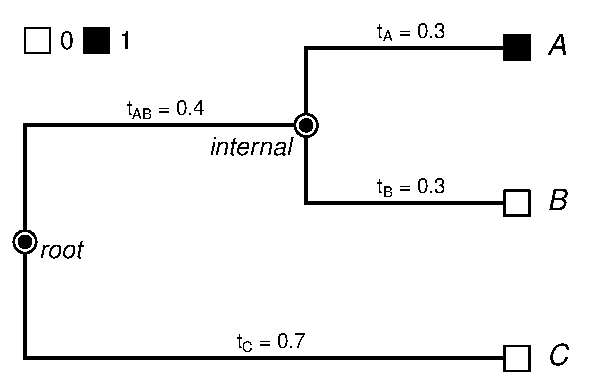
\includegraphics{Revell.AncestralReconstruction_files/figure-latex/fig1-1.pdf}
\caption{\label{fig:fig1}A simple, three-taxon, rooted phylogeny with two trait values of a discrete character (0 and 1) mapped at the tips of the tree. The two nodes of the tree (labeled \emph{root} and \emph{internal}, respectively) in whose states we might be interested in are indicated on the figure, as are the lengths of the four branches of the tree. See main text for more details.}
\end{figure}

Figure 1 shows a simplified rooted phylogeny with three terminal taxa (\emph{A}, \emph{B}, and \emph{C}) and two observed levels (0 and 1) of a discrete phenotypic trait. To compute the probability of the observed data at the tips of this tree under our Markov chain (M\emph{k}) model, we might begin by calculating \(\mathbf{P}_{t=0.4}\), \(\mathbf{P}_{t=0.3}\), and \(\mathbf{P}_{t=0.7}\) for our transition matrix \textbf{Q}. If we were to do so, we'd obtain the following three values.\footnote{Our tree has a total of four edges, but two of them have exactly the same total length of $t = 0.3$ (Figure 1).}

\[\mathbf{P}_{t=0.4} = \exp({\mathbf{Q} \times 0.4}) = \begin{bmatrix}0.926 & 0.074\\0.074 & 0.926\end{bmatrix}\]

\[\mathbf{P}_{t=0.3} = \exp({\mathbf{Q} \times 0.3}) = \begin{bmatrix}0.943 & 0.057\\0.057 & 0.943\end{bmatrix}\]

\[\mathbf{P}_{t=0.7} = \exp({\mathbf{Q} \times 0.7}) = \begin{bmatrix}0.878 & 0.122\\0.122 & 0.878\end{bmatrix}\]

Now, with these probability matrices in hand, we can proceed on to measuring the total probability of the data at the tips of the tree of Figure 1. To do this, one more probability that we need to consider is the (prior) probability that the global root of the tree was in condition 0 or condition 1 -- normally given as \(\pi_{0}\) and \(\pi_{1}\), respectively. There are various ways we might set \(\pi\) (see FitzJohn et al. 2009; Yang 2014; Revell and Harmon 2022). For simplicity here, I'll just say \(\pi_{0} = \pi_{1} = 0.5\) (a `flat' root prior); however, identifying a suitable root prior (\(\mathbf{\pi}\)) has been the subject of more substantive discussion elsewhere (FitzJohn et al. 2009; Yang 2014).

Having set \(\mathbf{\pi}\), we can compute the total probability of our data by summing the probability of our tip data (\emph{A} in condition 1, \emph{B} in 0, and \emph{C} in 0, shown here as \(P(1,0,0)\)), across all four possible combinations of states at the root and internal nodes of our tree, respectively: 0 \& 0, 0 \& 1, 1 \& 0, and 1 \& 1.

\[\begin{aligned}
P(1,0,0) &= \pi_{0} \times P(0|0,t_{AB}) \times P(1|0,t_{A}) \times P(0|0,t_{B}) \times P(0|0,t_{C})\\ 
            & + \pi_{0} \times P(1|0,t_{AB}) \times P(1|1,t_{A}) \times P(0|1,t_{B}) \times P(0|0,t_{C})\\
            & + \pi_{1} \times P(0|1,t_{AB}) \times P(1|0,t_{A}) \times P(0|0,t_{B}) \times P(0|0,t_{C})\\
            & + \pi_{1} \times P(1|1,t_{AB}) \times P(1|1,t_{A}) \times P(0|1,t_{B}) \times P(0|1,t_{C})\\
            & = 0.0267
\end{aligned}\]

In which \(P(1|0,t_{A})\) is the (1,2)th element of \(\mathbf{P}_{t=0.3}\), \(P(0|0,t_{C})\) is the (2,2)th element of \(\mathbf{P}_{t=0.7}\), and so on (Yang 2014; Harmon 2019).

After we calculate all the relevant quantities of our equation, we should find that the total probability of our data on this tree is 0.0267, given our transition matrix (\textbf{Q}) and modeled process.\footnote{Importantly, this is the probability of observing the data pattern [1, 0, 0] given our tree and matrix \textbf{Q}, not the probability of the tree or \textbf{Q}. That means that if we were to identify all possible data patterns ([0, 0, 0], [0, 0, 1], and so on), compute their probabilities, and then sum these quantities, this sum should be equal to 1.0.} In this case, for demonstrative purposes only, I've explicitly enumerated all of the possible internal node and root states of our tree; however, this would become very onerous for even a modestly-sized phylogeny of five or ten operational taxa.\footnote{Indeed, it's virtually impossible for larger trees.} Fortunately, Felsenstein (1981) described a highly efficient `pruning'\footnote{Felsenstein's procedure is called a pruning algorithm because it proceeds in a ``post-order'' fashion -- that is, from the tips towards the root of the tree -- performing a calculation based only on the descendant subtree of each internal node, pruning this subtree out of the phylogeny, and then using the computed quantities for the next, more rootward calculation.} algorithm to compute this exact probability.

So far we've treated \textbf{Q} as if it were fixed. In practice, we invariably \emph{estimate} \textbf{Q}, typically by identifying the value of \textbf{Q} that maximizes the probability of our data given the tree: our Maximum Likelihood estimate, by definition (Pagel 1994; Lewis 2001; Revell and Harmon 2022). Obviously, it makes little sense to try to estimate \textbf{Q} from a tree containing only three observations! Consequently, for now we'll continue using this same fixed value of \textbf{Q}, but we should at the same time keep in mind that in any empirical studies \textbf{Q} is nearly invariably estimated from the same data that are being used to reconstruct ancestral states -- rather than set to a fixed value or known \emph{a priori}.

\subsection{Marginal vs.~joint (and local vs.~global) estimation}\label{marginal-vs.-joint-and-local-vs.-global-estimation}

An important consideration when discussing ancestral state reconstruction of discrete characters is the distinction between what are known as \emph{marginal} and \emph{joint} reconstruction (Yang 2006; Revell and Harmon 2022).\footnote{In theory, the same distinction could be made for continuous traits -- except that, in that case, our marginal and joint estimates are the same!} Marginal reconstruction involves proceeding from node to node on the phylogeny, and, at each node, computing the probability of observing the tip data of our tree conditioned on fixing the node we've visited to each one of the set of distinct values of our trait. This set of probabilities, referred to as marginal likelihoods, are normally rescaled such that they add to 1.0,\footnote{Doing so merely entails dividing each by the total likelihood.} at which point they're frequently referred to as the node \emph{marginal scaled likelihoods}. Yang (2006, 2014) has pointed out that these scaled likelihoods are also a type of empirical Bayes posterior probability.\footnote{Empirical Bayes estimation involve fixing one level of the Bayesian heirarchy -- in this case, the value of our transition matrix \textbf{Q} -- to its most likely value, and then computing our posterior probabilities while conditioning on this fixed level.} They can thus be validly interpreted as the (posterior) probabilities that each node is in each of the observed character states, whilst conditioning on our fitted transition process, \textbf{Q}. Joint reconstruction, on the other hand, involves identifying the set of all internal node values (among all possible such sets) that maximizes the probability of our data. As observed by Yang (2006), these needn't necessarily be the set of states with the highest marginal scaled likelihoods!

In addition to marginal vs.~joint ancestral state reconstruction, another potentially important distinction that occasionally appears in the literature is between \emph{global} and \emph{local} reconstruction (Pagel 1999). In this case, the difference between global and local involves the estimation of \textbf{Q} itself. Under global reconstruction, we estimate our transition matrix \textbf{Q} (using, say, Maximum Likelihood) only \emph{once} based on the phylogeny and all the data at the tips of the tree, without any particular assumption about the value of our character at any individual node of the phylogeny (apart from the root -- see my discussion of the root prior, \(\pi\), above). We then proceed to undertake ancestral state reconstruction while holding \textbf{Q} constant at this value (Yang et al. 1995; Koshi and Goldstein 1996; Schluter et al. 1997; Pagel 1999; Yang 2006; Revell and Harmon 2022). Under \emph{local} ancestral state reconstruction, on the other hand, \textbf{Q} is co-estimated separately with every internal node state value (Pagel 1999). Although Pagel (1999) argued fairly persuasively for the merits of local ancestral state reconstruction of discrete traits, the global method (in which \textbf{Q} is held constant) has nonetheless come to predominate ancestral state estimation of discrete traits (Revell and Harmon 2022).\footnote{Indeed, in earlier drafts of this article I didn't even include this discussion!} I'll focus on global ancestral state estimation in the sections that follow; however, the reader can keep in mind (if they like) that local estimation would merely involve substituting a different value of \textbf{Q} for each state or set of states\footnote{Normally that value of \textbf{Q} that maximized the likelihood, conditioned on that state or set of states.} at internal nodes during estimation. All other calculations are unchanged from what's shown below.

\subsection{Marginal ancestral state estimation}\label{marginal-ancestral-state-estimation}

Marginal ancestral state reconstruction involves traversing the tree and at each node calculating the probability of the tip data in our tree under our model, conditioned on our current node being in each of our character levels (Pagel 1999; Yang 2006). These `marginal' probabilities are then normalized by dividing by their sum at each node, at which point they can be interpreted as the (empirical Bayes posterior) probability that each node is in each state of the character (Yang 2006; Revell and Harmon 2022). Since we've already calculated all the relevant quantities for our example of Figure 1, let's proceed and evaluate first the marginal likelihoods at the root, then the marginal likelihoods for our single internal node.

\[\begin{aligned}
P(root=0) & = \pi_{0} \times P(0|0,t_{AB}) \times P(1|0,t_{A}) \times P(0|0,t_{B}) \times P(0|0,t_{C})\\ 
            & + \pi_{0} \times P(1|0,t_{AB}) \times P(1|1,t_{A}) \times P(0|1,t_{B}) \times P(0|0,t_{C})\\
            & = 0.5 \times 0.0434 + 0.5 \times 0.0035\\
            & = 0.0234
\end{aligned}\]

\[\begin{aligned}
P(root=1) & = \pi_{1} \times P(0|1,t_{AB}) \times P(1|0,t_{A}) \times P(0|0,t_{B}) \times P(0|1,t_{C})\\
            & + \pi_{1} \times P(1|1,t_{AB}) \times P(1|1,t_{A}) \times P(0|1,t_{B}) \times P(0|1,t_{C})\\
            & = 0.5 \times 0.0005 + 0.5 \times 0.0060 \\
            & = 0.0033
\end{aligned}\]

Here \(P(root = 0)\) gives the probability of our observed data (conditioning on \textbf{Q}), given that the root is in state 0; while \(P(root = 1)\) gives the probability of our data, given that the root is in state 1.\footnote{Importantly, $P(root = 0)$ and $P(root = 1)$ \emph{do not} give the probability that the root state was in condition 0 or condition 1, respectively. If they did, then we would expect their values to add to 1.0! Just to reiterate what is also stated in the main text, they give the probabilities of \emph{our tip data} (under the model) given that the root is in condition 0 or in condition 1, respectively.} If these two quantities are rescaled by their sum, however (which is also, recall, the total likelihood), we obtain the marginal scaled likelihoods for states 0 and 1 of \(P(0,1) = [0.878, 0.122]\) at the root node of the tree.

Now let's repeat the same procedure for the single internal node of our phylogeny of Figure 1.

\[\begin{aligned}
P(internal=0) & = \pi_{0} \times P(0|0,t_{AB}) \times P(1|0,t_{A}) \times P(0|0,t_{B}) \times P(0|0,t_{C})\\ 
            & + \pi_{1} \times P(0|1,t_{AB}) \times P(1|0,t_{A}) \times P(0|0,t_{B}) \times P(0|1,t_{C})\\
            & = 0.5 \times 0.0434 + 0.5 \times 0.0005 \\
            & = 0.0219
\end{aligned}\]

\[\begin{aligned}
P(internal=1) & = \pi_{0} \times P(1|0,t_{AB}) \times P(1|1,t_{A}) \times P(0|1,t_{B}) \times P(0|0,t_{C})\\
            & + \pi_{1} \times P(1|1,t_{AB}) \times P(1|1,t_{A}) \times P(0|1,t_{B}) \times P(0|1,t_{C})\\
            & =  0.5 \times 0.0035 + 0.5 \times 0.0060 \\
            & = 0.0047
\end{aligned}\]

Once again, if these two quantities are rescaled by their sum, which is also the total likelihood (just as it was for the root node), we'll have the marginal scaled likelihoods for conditions 0 and 1 of \(P(0,1) = [0.822, 0.178]\). Figure 2a gives the marginal ancestral state reconstruction of our tree and data in Figure 1,\footnote{Mapped to the corresponding nodes of the tree using a pie diagram, as is very commonly done in empirical studies that use marginal ancestral state reconstruction.} conditioned on the value of \textbf{Q} indicated earlier in the article.

\begin{figure}
\centering
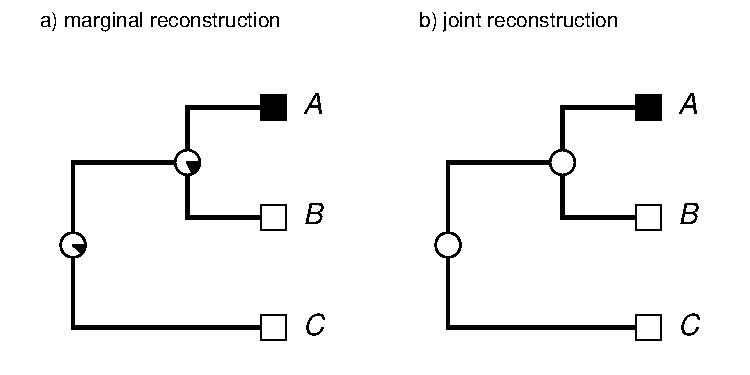
\includegraphics{Revell.AncestralReconstruction_files/figure-latex/fig2-1.pdf}
\caption{\label{fig:fig2}(a) Marginal ancestral state reconstruction based on the tree and data of Figure 1. (b) Joint ancestral reconstruction. Both reconstructions assume a constant value of \textbf{Q}, as indicated in the text. See main text for more details.}
\end{figure}

As for computing the total likelihood, above, for demonstrative purposes I have enumerated all the terms of each marginal likelihood. This would quickly become prohibitively complicated for even modestly-sized phylogenies so in practice computer implementations of marginal ancestral state reconstruction use one of various fast algorithms based on pruning to compute these quantities (Felsenstein 1981; Yang 2006).

\subsection{Joint reconstruction}\label{joint-reconstruction}

The other type of ancestral state reconstruction that we might perform under the M\emph{k} model, in addition to the method of marginal ancestral state reconstruction that we just learned, is what's typically referred to as \emph{joint} reconstruction (Yang 2006; Revell and Harmon 2022). In this case, our estimated ancestral states are merely the set of such states that jointly maximize the probability of our data at the tips of the tree.

In our example from Figure 1, there are a total of four possible \emph{sets} of states at the two nodes of the phylogeny: \([0,0]\), \([0,1]\), \([1,0]\), and \([1,1]\).\footnote{In general, there will be a number $k^m$ of such sets for $k$ character levels and $m$ nodes. It goes without saying that computer implementations of joint ancestral state reconstruction do not comprehensively enumerate all possible node state combinations to find the set that maximizes the likelihood!} Uncoincidentally, these four sets of states correspond to the four terms of our equation for the probability of our data (\(P(0,0,1)\)), above. In other words:

\[\begin{aligned}
P([0,0]) & = \pi_{0} \times P(0|0,t_{AB}) \times P(1|0,t_{A}) \times P(0|0,t_{B}) \times P(0|0,t_{C}) = 0.0217\\ 
P([0,1]) & = \pi_{0} \times P(1|0,t_{AB}) \times P(1|1,t_{A}) \times P(0|1,t_{B}) \times P(0|0,t_{C}) = 0.0017\\
P([1,0]) & = \pi_{1} \times P(0|1,t_{AB}) \times P(1|0,t_{A}) \times P(0|0,t_{B}) \times P(0|1,t_{C}) = 0.0002\\
P([1,1]) & = \pi_{1} \times P(1|1,t_{AB}) \times P(1|1,t_{A}) \times P(0|1,t_{B}) \times P(0|1,t_{C}) = 0.0030\\
\end{aligned}\]

Here, \(P([0,0])\) gives the probability of our data at the tips of the tree, conditioning on both the root and single internal node of the tree being in states 0 and 0, respectively. The same interpretation can be made of \(P([0,1])\), \(P([1,0])\), and so on. From this set of values we can see that the combination of states that jointly maximizes the probability of our data are \([0,0]\) -- in other words, condition 0 at both the root and single internal node of the tree (Figure 1). This set thus becomes our \emph{joint} Maximum Likelihood ancestral state estimate. We could also imagine rescaling the set of probability values by their sum and reporting the probabilities of each set of states conditioned on \textbf{Q} -- though this is not typically undertaken in joint reconstruction. Figure 2b illustrates the joint reconstruction from our tree and data of Figure 1.

\subsection{Stochastic character mapping}\label{stochastic-character-mapping}

In addition to joint and marginal reconstruction, a third important and popular method of ancestral state estimation under the M\emph{k} model is the procedure called stochastic character mapping (Huelsenbeck et al. 2003; Bollback 2006; Revell and Harmon 2022; Revell 2024).\footnote{Stochastic character mapping originally derives from a closely related approach called `mutational mapping' (Nielsen 2002) and was first generalized to phenotypic traits by Huelsenbeck et al. (2003).} Under stochastic character mapping, complete character histories (including character state changes along the branches of the tree) are randomly\footnote{In other words, ``stochastically,'' hence the name of the method.} sampled from their probability distribution under a model.

Stochastic character mapping is a computationally intensive method. The most efficient algorithm to generate a single stochastic character map minimally involves two traversals of the tree. The first of these is a post-order (tip to root) ``pruning'' traversal in which a set of conditional likelihoods of each subtree is calculated for each node of the tree. These are the set of marginal likelihoods, under our model, for \emph{only} the data descended from a given node.\footnote{Note that if we generate more than one stochastically mapped history for a given tree and value of \textbf{Q}, as we nearly invariably should, these values can be recycled across simulations and do not need to be recomputed.} Once the root node is reached, these calculated quantities \emph{also} correspond to the marginal likelihoods at this node and sum to the total probability of our data under the model. A root state is randomly sampled with probability equal to its marginal scaled likelihoods.

Next, we undertake a pre-order tree traversal. Looking at each daughter node from the root, we first calculate a set of updated probablities (\textbf{p}) that each of the two or more daughters is in each state of our character. For each daughter, this vector of probabilities, \textbf{p}, is simply equal to the \emph{i}th row of the exponentiated product of \textbf{Q}, the transition matrix, and the elapsed time of the daughter edge, multiplied element-wise\footnote{Also known as the Hadamard product.} by the vector of conditional likelihoods of the subtree for that node -- the values that we computed in our prior post-order tree traversal. In other words, \(\mathbf{p} = \exp(\mathbf{Q}t)_{i\cdot} \odot \mathbf{L}\), in which the subscript \(i\cdot\) indicates the \emph{i}th row of \(\exp(\mathbf{Q}t)\), \(\odot\) is the element-wise vector product, and \textbf{L} is a vector of conditional likelihoods.

We then proceed to the daughter node and randomly sample a state for it according to the probabilities given by \textbf{p}. We use simulation and rejection sampling to obtain a discrete character character history along that edge consistent with our sampled parent and daughter node states. Finally, we recursively traverse the phylogeny in a post-order (root to tip) fashion repeating this procedure for each pair of parent and daughter nodes.\footnote{Of course, if the daughter node is a tip then typically the state will be known rather than sampled probabilistically, but our procedure is otherwise identical.} Figure 3 gives an example of ten stochastic character histories, given our phylogeny and data of Figure 1 and the \textbf{Q} transition matrix of our previous sections in which \(q_{0,1} = q_{1,0} = 0.2\). Normally, we'd generate many more than ten stochastic character histories!

\begin{figure}
\centering
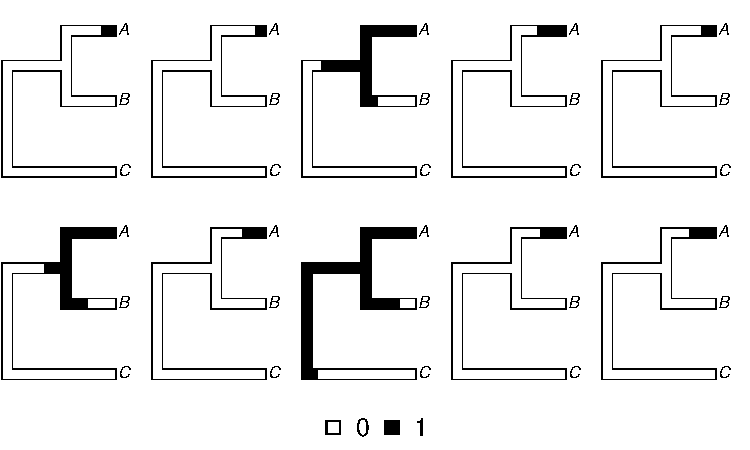
\includegraphics{Revell.AncestralReconstruction_files/figure-latex/fig3-1.pdf}
\caption{\label{fig:fig3}A set of ten stochastic character maps for the tree and data of Figure 1. As in Figure 2, these stochastic character histories were sampled in proportion to their probability using a constant value of the transition matrix \textbf{Q}. See main text for more details.}
\end{figure}

A single stochastic character map contains almost no information about evolutionary history, but a set of many such maps can be used to measure the posterior probabilities that each node is in each state of our character, as well as to generate an estimate of the probability distribution of the number of changes of each type on the tree. Indeed, when a single, fixed value of \textbf{Q} is used for stochastic mapping, the relative frequencies of each state at each node and the marginal scaled likelihoods from our previous section should exactly converge as the number of stochastic simulations goes to \(\infty\).\footnote{Though normally they will be highly similar after 100 or 1,000 simulations.} An advantage of stochastic character mapping, however, is that it also allows us to take into account uncertainty in the transition process represented by \textbf{Q}. For example, it's straightforward to sample \textbf{Q} from its Bayesian posterior distribution using MCMC, or to use a set of transition processes in proportion to their weight based on model comparison (e.g., Revell and Harmon 2022; Revell 2024).

\subsection{Empirical examples}\label{empirical-examples}

\subsubsection{Marginal reconstruction: Diel activity pattern in primates}\label{marginal-reconstruction-diel-activity-pattern-in-primates}

To demonstrate marginal reconstruction, we'll study diel activity pattern\footnote{Coded as `nocturnal,' `diurnal,' and `cathemeral' (active randomly during the day or night) in these data.} among 90 species of primates. The phylogeny and data for this example come from Kirk and Kay (2004; but see a similar analysis using different data in Santini et al. 2015).

Our first step, in this case, will be to fit a set of four M\emph{k} models to our tree and data. We can begin with a very simple model in which we assume that the rates of transitions between all three pairs of our states (nocturnal \(\leftrightarrow\) diurnal, nocturnal \(\leftrightarrow\) cathemeral, and diurnal \(\leftrightarrow\) cathemeral) are all equal one to the other, and in both directions. This model is called the `equal-rates' (ER) model and our matrix, \textbf{Q}, will have just one parameter to be estimated. Next, we might proceed to fit a model in which the backward and forward transition rates between each pair of states are equal (one to the other), but different for each character state pair. This is called the `symmetric' (SYM) model and has a total of three parameters. We'll fit a model in which every transition rate in each direction is permitted to assume a different rate. This is called the `all-rates-different' (ARD) model, and our \textbf{Q} matrix for this model will include a total of six parameters to be estimated.\footnote{In general the ARD model has a total of $k \times (k-1)$ parameters for $k$ states.} Lastly, we'll fit a model in which we imagine that the cathemeral condition is intermediate between the nocturnal and diurnal activity states, whereby any lineage evolving from one to the other must first pass through the state of cathemeral diel activity. This set of fitted models, and their AIC values and Akaike weights, is given in Figure 4.

\begin{figure}
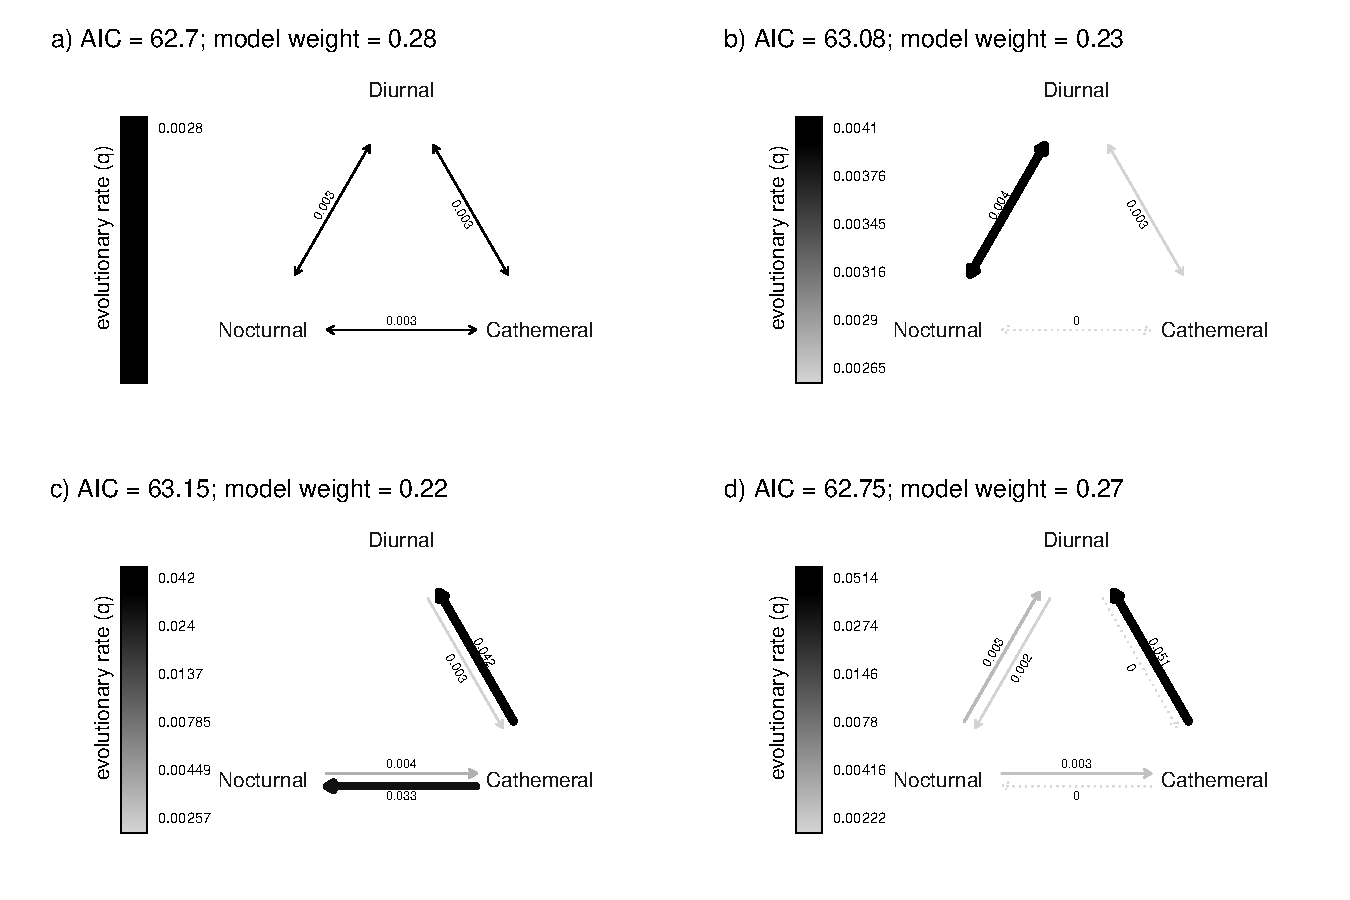
\includegraphics[width=1\linewidth]{Revell.AncestralReconstruction_files/figure-latex/fig4-1} \caption{A set of fitted M\emph{k} models for the evolution of diel activity pattern in primates. (a) The equal-rates (ER) model. (b) The symmetric (SYM) model. (c) An ordered model in which the cathemeral state is assumed to be intermediate between the other two conditions. Finally, (d) the all-rates-different (ARD) model. These models involve the estimation of 1, 3, 4, and 6 parameters, respectively. Note that the legend color gradient differs for each figure panel. Model-support and Akaike weights are indicated in each panel header. The data and phylogeny for this analysis derive from Kirk and Kay (2004). See main text for more details.}\label{fig:fig4}
\end{figure}

Since the weight of evidence is fairly even across each in our set of four models\footnote{This is a bit unusual, in my experience. Typically, one model tends to be substantially better-supported than the rest!}, I elected to use model-averaged marginal ancestral state estimation.\footnote{Model-averaging simply involves taking the Akaike weights, multiplying them by the marginal scaled likelihoods for each model, and then summing across models (Revell, 2024).} The resultant marginal ancestral states are shown in Figure 5. They reveal that the common ancestor was most likely nocturnal (under our fitted model), and also suggest multiple transitions to diurnal diel activity pattern in different parts of the primate tree of life (Figure 5).

\begin{figure}
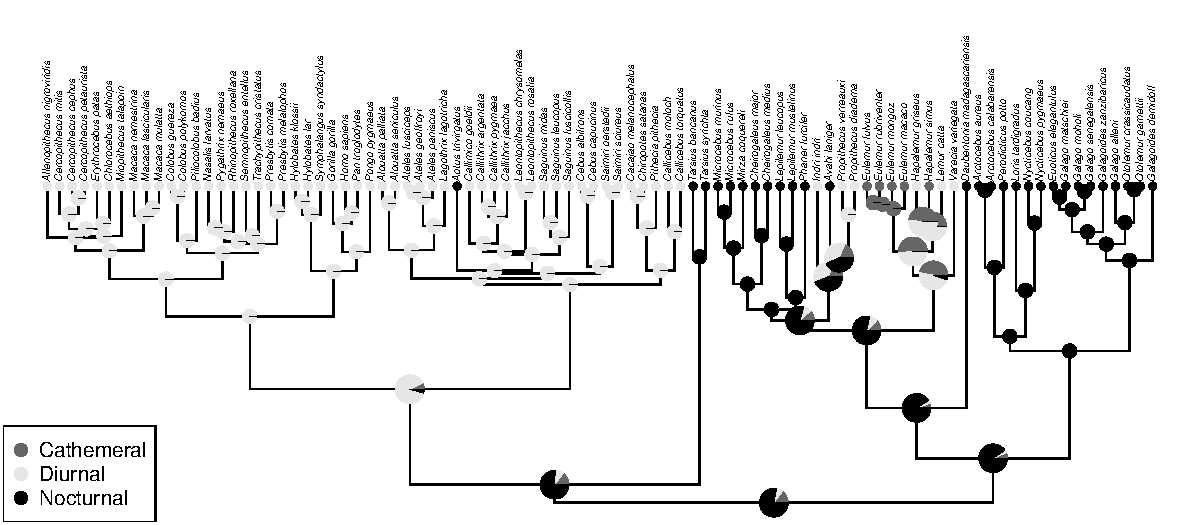
\includegraphics[width=1\linewidth]{Revell.AncestralReconstruction_files/figure-latex/fig5-1} \caption{Model-averaged marginal ancestral state reconstruction of diel activity pattern in primates, integrating over the four models of Figure 4 in proportion to their Akaike weights. Nodes in which no single condition had a model-averaged marginal scaled likelihood > 0.95 are shown in larger size. The data and phylogeny for this analysis derive from Kirk and Kay (2004). See main text for more details.}\label{fig:fig5}
\end{figure}

\subsubsection{Joint reconstruction: Tail spines in lizards}\label{joint-reconstruction-tail-spines-in-lizards}

To illustrate joint reconstruction, we'll use a phylogeny from Pyron et al. (2013) along with a dataset of tail spine presence and absence in lizards originally published by Ramm et al. (2020). To commence, we can fit a set of just two M\emph{k} models for this binary trait: the ER model, in which the back-and-forth transitions between our two states are forced to take place at the same rate; and the ARD model in which they can differ.\footnote{We might have also considered two irreversible models: one in which tail spines can \emph{only} be gained in our tree; and another in which they are only lost. In this case, doing so would not have substantively changed our results.}

\begin{table}

\caption{\label{tab:unnamed-chunk-22}Estimated transition rates, log-likelihood, number of parameters, AIC, and model weights for two different discrete character evolution models for the evolution of the presence or absence of tail spines in lizards. The phylogeny used in this analysis is based on Pyron et al. (2013), and the data were compiled by Ramm et al. (2020). See main text for more details.}
\centering
\begin{tabular}[t]{l|r|r|r|r|r|r}
\hline
  & $q_{0,1}$ & $q_{1,0}$ & log(L) & d.f. & AIC & weight\\
\hline
ER model & 0.00152 & 0.00152 & -123.5618 & 1 & 249.1235 & 0.0688\\
\hline
ARD model & 0.00059 & 0.01112 & -119.9564 & 2 & 243.9129 & 0.9312\\
\hline
\end{tabular}
\end{table}

The results from this analysis are shown in Table 1. Our analysis indicates much higher model weight (0.93 vs.~0.07) for the ARD compared to the ER model. Consequently, we used only this model for our subsequent joint ancestral state reconstruction, given in Figure 6.\footnote{An interesting `footnote' (get it?) to this result is that the ML joint reconstruction at the global root of the tree is `non-spiny,' but in an analogous marginal reconstruction the most \emph{probable} condition for the same node was `spiny.' We haven't included this analysis here, but the reader is encouraged to download the data and discover this for themselves!}

\begin{figure}
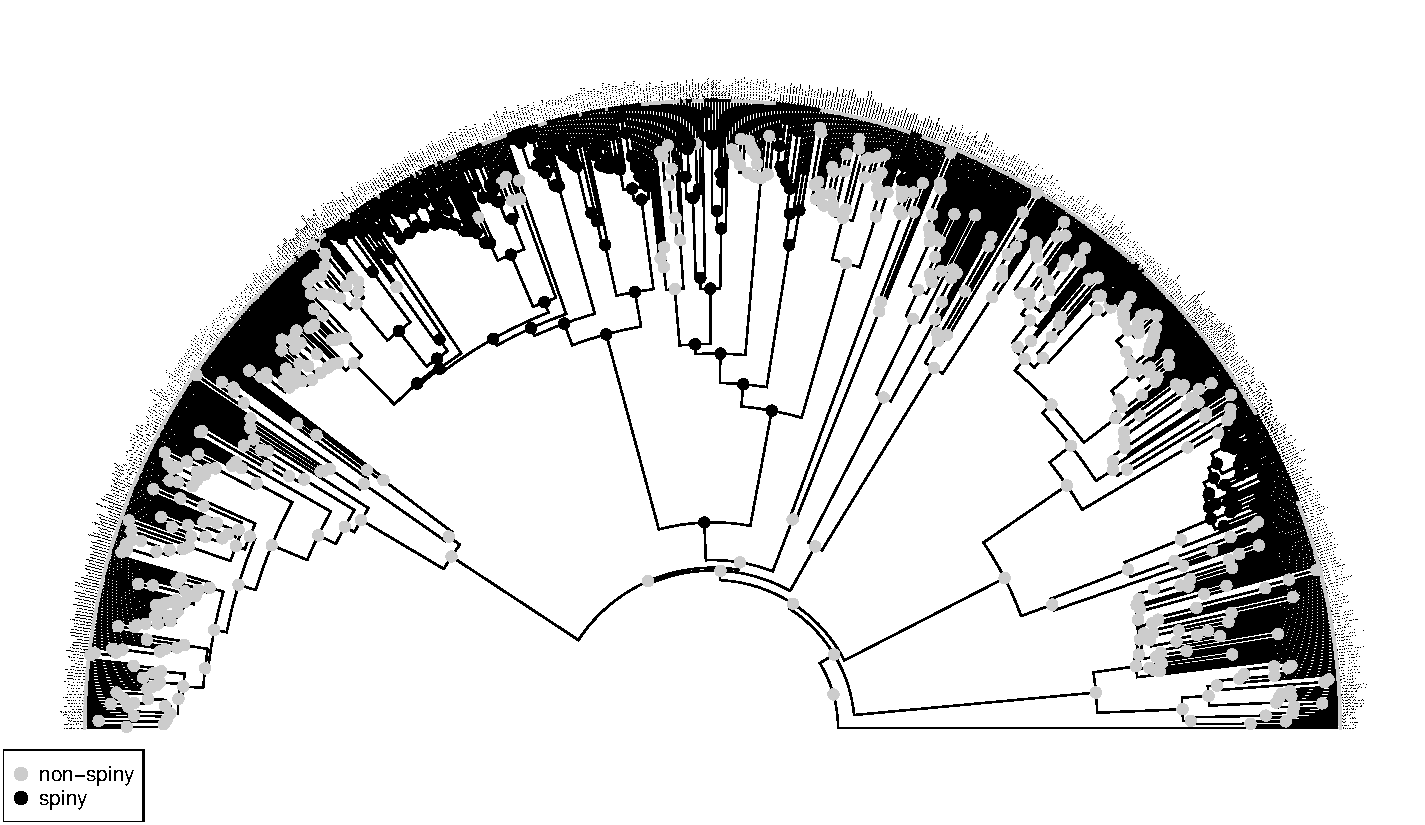
\includegraphics[width=1\linewidth]{Revell.AncestralReconstruction_files/figure-latex/fig6-1} \caption{Joint reconstruction of the presence and absence of tail spines on a phylogeny of 658 species of lizards. Reconstruction was performed under the best-supported M\emph{k} model which featured unequal back and forth transition rates between the two different character levels of the tree (the ARD model; Table 1). The phylogeny and data for this analysis derive from Pyron et al. (2013) and Ramm et al. (2020), respectively. See main text for more details.}\label{fig:fig6}
\end{figure}

Joint reconstruction involves a key difference in interpretation compared to marginal reconstruction. Now, we can no longer point to a particular node and say that the most probable state is ``spiny'' or ``non-spiny.'' Rather, we might say that ``in the most probable joint reconstruction, the ancestral condition at the global root was non-spiny,'' or something to that effect. Since researchers more often wish to be able to make specific statements about particular nodes,\footnote{Rather than the most probable set of conditions across \emph{all} nodes.} marginal reconstruction tends to be the much more popular of these two techniques among comparative biologists.

\subsubsection{Stochastic character mapping: Leaf armature in palms}\label{stochastic-character-mapping-leaf-armature-in-palms}

To demonstrate stochastic character mapping, I used a recent dataset and phylogeny published by Onstein et al. (2022). In this example, the phylogeny contains a total of 2,539 tree species from the family Arecaceae (the palms), and data for the presence of absence of leaf armature (spines, hooks, or prickles on the palm leaves) for all but 120 of these taxa. The trait data of this study were compiled by Onstein et al. (2022) from the PalmTraits 1.0 database (Kissling et al. 2019), and the palm phylogeny is derived from an earlier tree by Faurby et al. (2016).

To begin, I re-coded all data deficient species (which had been left out by Onstein et al. 2022) as ambiguous\footnote{Coding for ambiguity simply involves observing, \emph{a priori}, that an ambiguous tip could equally likely be in one condition or the other. The total probability of the data then becomes the sum of the probability conditioning first on the tip state being in one state and then in the other. This total probability can be computed efficiently via the pruning algorithm of Felsenstein (1981).} for the trait of leaf armature, and then I proceeded to fit a total of four M\emph{k} trait evolution models: the ER model, the ARD model, and two irreversible models (one in which leaf armature could be acquired but not lost, and a second in which the reverse was true). A summary of parameter estimates and model support is given in Table 2. I found almost no support for the two irreversible models, but roughly similar weights of evidence for the two different reversible models: ER and ARD (Table 2).

\begin{table}

\caption{\label{tab:unnamed-chunk-28}Estimated transition rates, log-likelihood, number of parameters, AIC, and model weights for four different discrete character evolution models for the evolution of the presence or absence of leaf armature in palms. The phylogeny and data for this analysis derive from Faurby et al. (2016), Kissling et al. (2019), and Onstein et al. (2022). See main text for more details.}
\centering
\begin{tabular}[t]{l|r|r|r|r|r|r}
\hline
  & $q_{0,1}$ & $q_{1,0}$ & log(L) & d.f. & AIC & weight\\
\hline
ER model & 0.00392 & 0.00392 & -431.5580 & 1 & 865.1161 & 0.57424\\
\hline
absent $\rightarrow$ present & 0.01162 & 0.00000 & -617.2943 & 1 & 1236.5886 & 0.00000\\
\hline
present $\rightarrow$ absent & 0.00000 & 0.01279 & -485.6286 & 1 & 973.2573 & 0.00000\\
\hline
ARD model & 0.00338 & 0.00471 & -430.8572 & 2 & 865.7145 & 0.42576\\
\hline
\end{tabular}
\end{table}

I next generated 500 stochastic character maps in which each of the four models were sampled randomly with probabilities given by their relative model weights (Table 2). Note that the sampling algorithm and total sample size of stochastic character maps is such that it ensures almost no irreversible (absent \(\rightarrow\) present or present \(\rightarrow\) absent) stochastic character histories will be sampled. A single, randomly chosen stochastic mapped tree is shown in Figure 7.

\begin{figure}
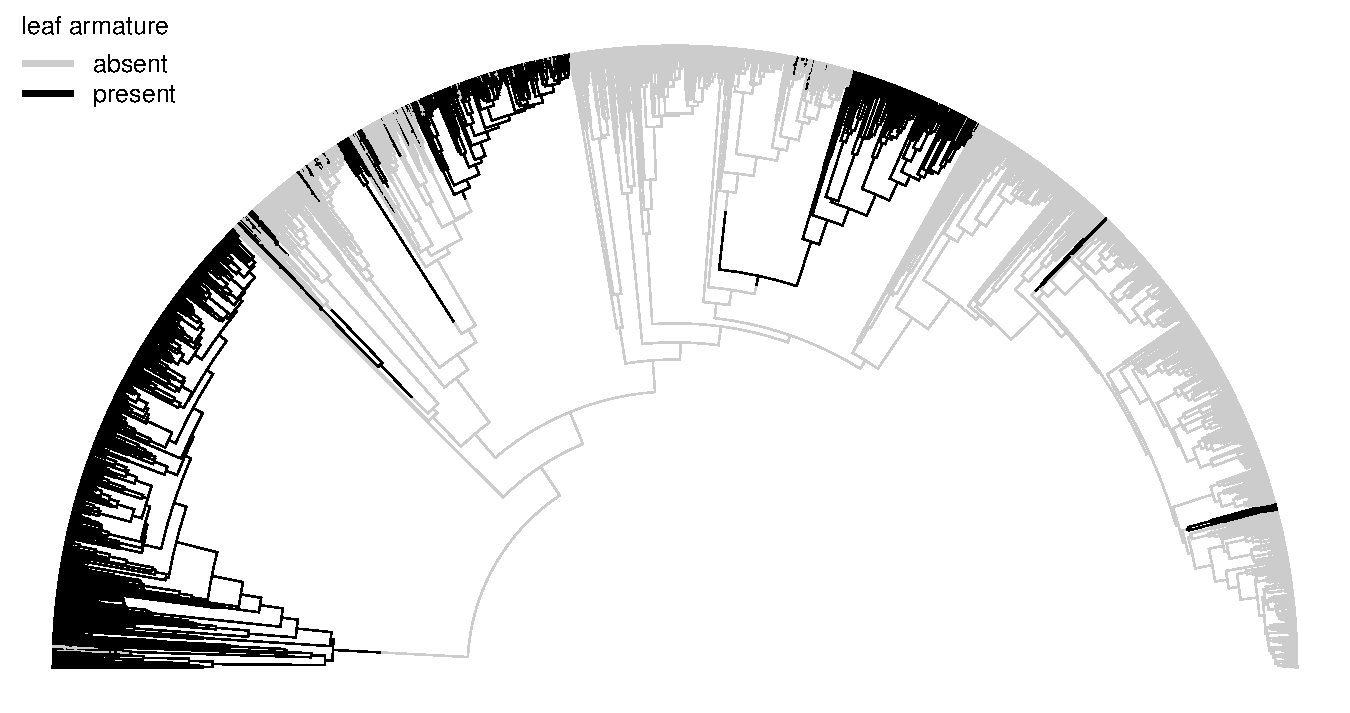
\includegraphics[width=1\linewidth]{Revell.AncestralReconstruction_files/figure-latex/fig7-1} \caption{A single stochastically-sampled character history of the absence (grey) or presence (black) of leaf armature (spines or other defensive structures) in 2,539 species of palms. The phylogeny and data for this analysis derive from Faurby et al. (2016), Kissling et al. (2019), and Onstein et al. (2022). See main text for more details.}\label{fig:fig7}
\end{figure}

Normally, relatively little can be learned from a single, stochastic character history such as that shown in Figure 7. On the other hand, neither is anything to be gained by visualizing 500 such histories -- particularly for large phylogenetic trees! For this reason, various tactics have been proposed to summarize the results across a set of stochastic character maps (Revell 2013, 2024; Revell 2014b; Revell and Harmon 2022). Two such analyses are shown in Figure 8. In particular, Figure 8a shows a posterior density map (Revell 2013; Revell 2014b) obtained by measuring the relative frequency of each of the two states over our set of 500 stochastic simulations across all edges and nodes of the tree. These frequencies give the posterior probabilities\footnote{These will be empirical Bayes posterior probabilities for a fixed value of \textbf{Q}; however, full Bayesian probabilities are also possible -- for example, if the \textbf{Q} matrix is sampled from its posterior probability distribution using MCMC.} along all of the edges and nodes of the phylogeny. Figure 8b, on the other hand, illustrates a visualization of the posterior probability distribution of the number of changes of each type on the phylogeny. These distributions are obtained simply by counting the changes in each of the 500 stochastically sampled character maps (e.g., Revell 2024).

\begin{figure}
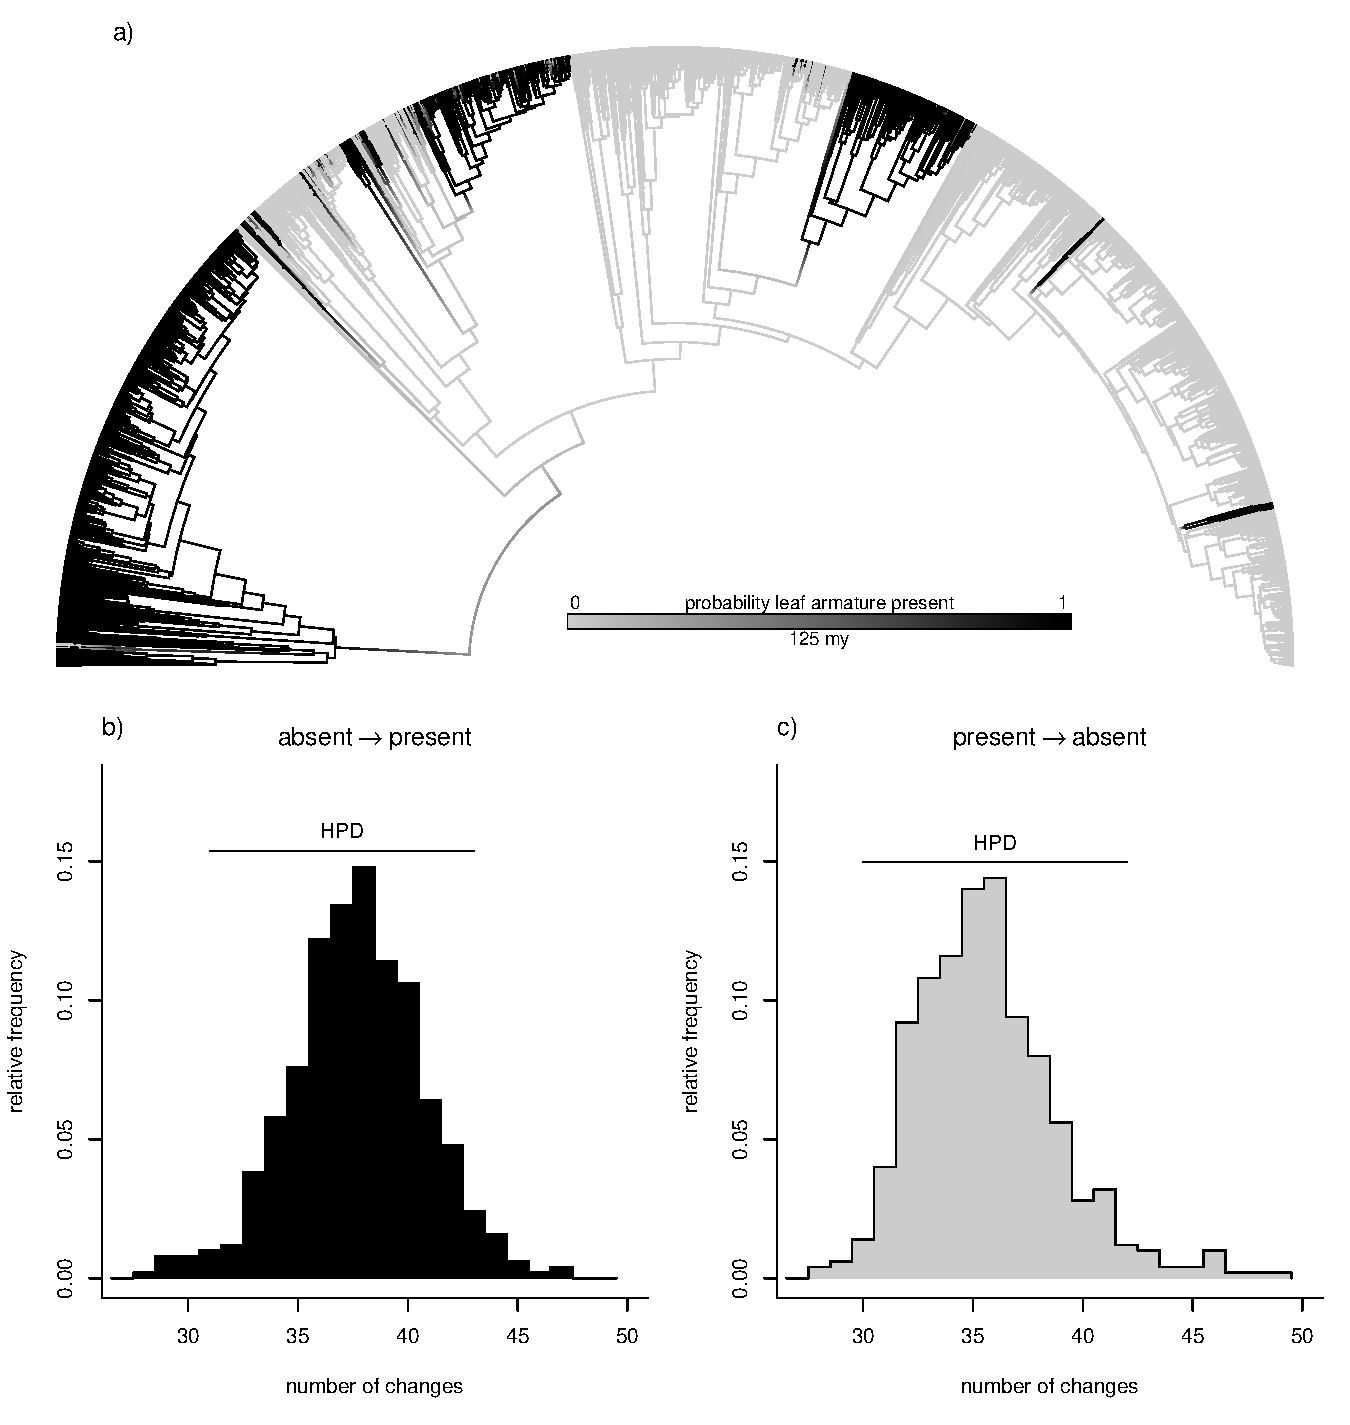
\includegraphics[width=1\linewidth]{Revell.AncestralReconstruction_files/figure-latex/fig8-1} \caption{(a) Probability density of the absence/presence of leaf armature based on 500 stochastic character mapping on a phylogenetic tree of 2,539 palm species. The four models of Table 2 were randomly sampled in proportion to their model weights following Revell (2024). Probability density of changes from leaf armature absent to present (b) and present to absent (c) from 500 stochastic character maps. The phylogeny and data for this analysis derive from Faurby et al. (2016), Kissling et al. (2019), and Onstein et al. (2022). See main text for more details.}\label{fig:fig8}
\end{figure}

\section{Continuous characters}\label{continuous-characters}

\subsection{The Brownian motion model}\label{the-brownian-motion-model}

The standard model employed to study the evolution of continuous traits, as well as (especially) to reconstruct their ancestral values, is one called the Brownian motion model (Felsenstein 1973; Felsenstein 1985; O'Meara et al. 2006; Harmon 2019). Brownian motion is a continuous time, directionless, random walk model (Harmon 2019; Revell and Harmon 2022). Under Brownian motion, successive evolutionary changes are independent and come from a Gaussian distribution with mean of 0 and variance of \(\sigma^2 \times t\), in which \(\sigma^2\) is the instantaneous rate of the Gaussian process and \(t\) is the elapsed time (Harmon 2019). Figure 9 shows a simulation of Brownian motion\footnote{Technically to create the visualization I discretized the depth of the tree into 200 units making this a discrete-time random walk, but the effect is the same.} evolution (Figure 9b) on the same simplified phylogenetic tree of three taxa that we saw earlier in the article (e.g., Figure 1), but in which I have re-colored the edges with different shades of gray (Figure 9a) so that they can be matched more easily with the Brownian trait evolution scenario (Figure 9b).

\begin{figure}
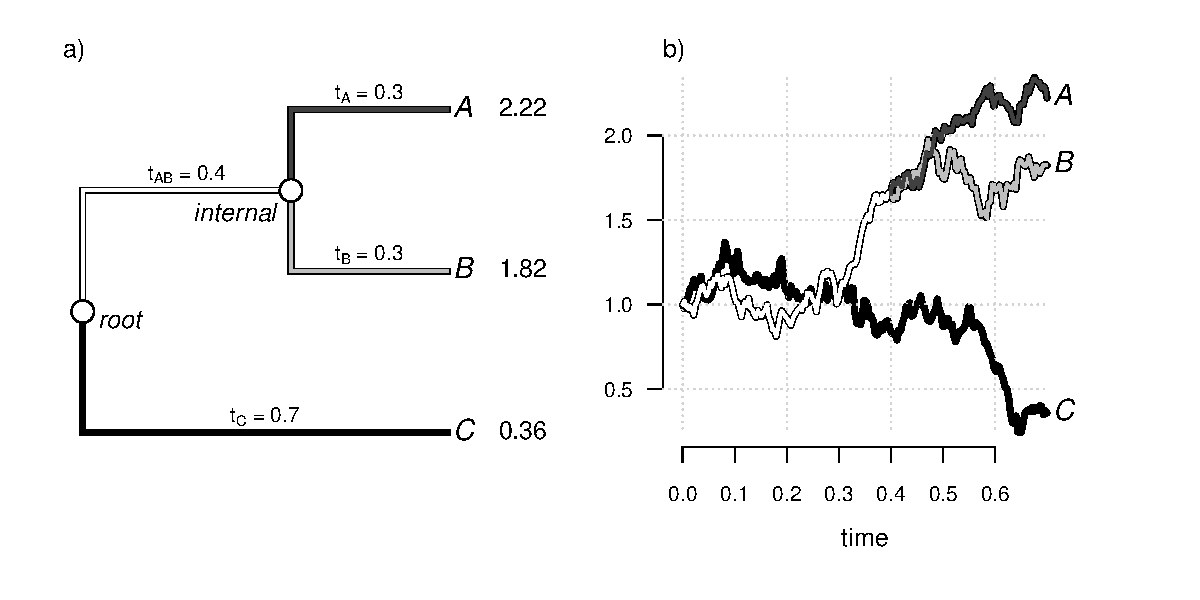
\includegraphics[width=1\linewidth]{Revell.AncestralReconstruction_files/figure-latex/fig9-1} \caption{(a) Three-taxon phylogenetic tree of Figure 1, but in which each edge of the tree has been plotted with a different color. (b) Single illustrative realization of Brownian motion evolution on the tree of figure panel (a). See main text for more details.}\label{fig:fig9}
\end{figure}

Brownian motion evolution will produce a realized trait vector of phenotypic values among species that has an expected value (\(\text{E}[x]\)) equal to the root state (\(x_0\)), and a multivariate normal distribution with variance equal to the total height of each tip above the root multiplied by the instantaneous Brownian rate, \(\sigma^2\) (O'Meara et al. 2006). In other words \(\mathbf{x} \sim \mathit{MVN}(x_0,\sigma^2\mathbf{C})\) in which \textbf{C} is an \(N \times N\) matrix (for \emph{N} tips in the tree), where each \emph{i},\emph{j}th element contains the height above the root of the most recent common ancestor of taxa \emph{i} and \emph{j}. This matrix, \textbf{C}, for our phylogeny of Figure 9a would be calculated as follows (Revell and Harmon 2022).

\[
\mathbf{C} = 
\begin{bNiceMatrix}[first-row,first-col]
& A & B & C \\
A & t_A + t_{AB} & t_{AB} & 0.0 \\
B & t_{AB} & t_B + t_{AB} & 0.0 \\
C & 0.0 & 0.0 & t_C
\end{bNiceMatrix} =
\begin{bNiceMatrix}[first-row,first-col]
& A & B & C \\
A & 0.7 & 0.4 & 0.0 \\
B & 0.4 & 0.7 & 0.0 \\
C & 0.0 & 0.0 & 0.7
\end{bNiceMatrix}
\]

To compute the probability density of a set of data (\(\mathbf{x}\)) at the tips of the tree for any particular value of \(\sigma^2\) and \(x_0\), we must evaluate the following density function.\footnote{If this expression seems familiar to some readers, they should not be surprised: it is just a typical multivariate normal probability density function!}

\[
P(\mathbf{x}) = \frac{\exp(-\frac{1}{2}[\mathbf{x}-x_0]'(\sigma^2\mathbf{C})^{-1}[\mathbf{x}-x_0])}{\sqrt{(2\pi)^N\times\det(\sigma^2\mathbf{C})}}
\]

Finding the set of values for \(x_0\) and \(\sigma^2\) that maximize the value of this expression would provide us with the Maximum Likelihood estimates of these model parameters (O'Meara et al. 2006; Revell and Harmon 2022).

\subsection{Ancestral state estimation under Brownian motion}\label{ancestral-state-estimation-under-brownian-motion}

Under Brownian motion evolution of our trait, not only are the tips distributed as a multivariate normal random variable, so are the values of internal nodes (Schluter et al. 1997; Rohlf 2001; Revell and Harmon 2022). To find those node values that maximize the probability of our tip data, \textbf{x}, we merely have to expand the matrix \textbf{C} to include one additional row and column for each (non-root) internal node of the tree. In our three-taxon phylogeny of Figure 9a there is only one such node (labeled ``\emph{internal}'') and our matrix \textbf{C} thus looks as follows.

\[
\mathbf{C} = 
\begin{bNiceMatrix}[first-row,first-col]
& A & B & C & internal \\
A & t_A + t_{AB} & t_{AB} & 0.0 & t_{AB} \\
B & t_{AB} & t_B + t_{AB} & 0.0 & t_{AB} \\
C & 0.0 & 0.0 & t_C & 0.0 \\
internal & t_{AB} & t_{AB} & 0.0 & t_{AB}
\end{bNiceMatrix} =
\begin{bNiceMatrix}[first-row,first-col]
& A & B & C & internal \\
A & 0.7 & 0.4 & 0.0 & 0.4 \\
B & 0.4 & 0.7 & 0.0 & 0.4 \\
C & 0.0 & 0.0 & 0.7 & 0.0 \\
internal & 0.4 & 0.4 & 0.0 & 0.4
\end{bNiceMatrix}
\]

To find the set of ancestral states under Brownian motion that maximize the probability of our observed data (our ML states), we simply identify the internal node values and root state (\(x_0\)) that jointly maximize the probability of the tip data given our model. Figure 10 gives a log-likelihood surface for the ancestral values at the root node of the tree (on the \emph{x}-axis) and the single internal node: showing the maximum likelihood values of \(x_0\) and \(x_\mathit{internal}\) to be 1.29 and 1.82, respectively. The figure also includes an illustrative course of numerical optimization on this likelihood surface, though this result would (naturally) depend on our starting value and specific optimization routine (Figure 10).

\begin{figure}
\centering
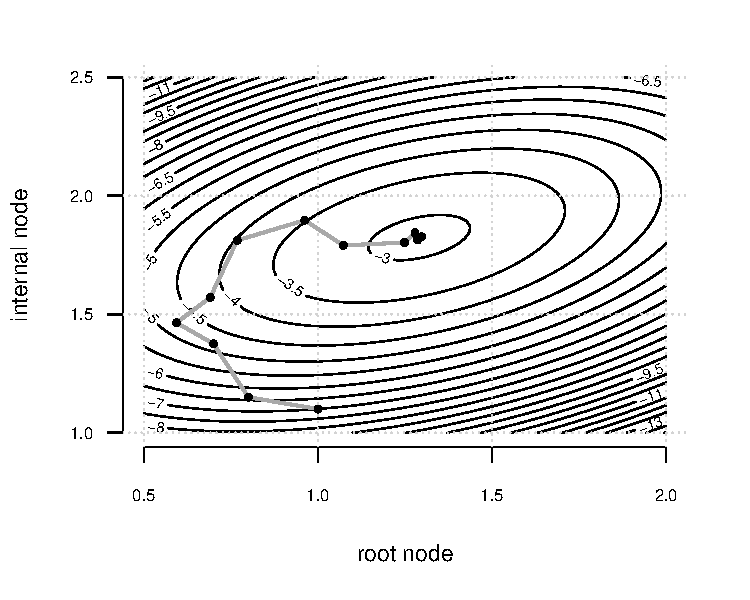
\includegraphics{Revell.AncestralReconstruction_files/figure-latex/fig10-1.pdf}
\caption{\label{fig:fig10}Log-likelihood surface for the numerical values of the root and internal nodes of the tree and phenotypic trait data of Figure 9. The grey line shows an illustration of numerical optimization on this surface which convergences to the Maximum Likelihood values of both node states. See main text for more details.}
\end{figure}

In practice, rapid algorithms have been identified to find the set of internal node values that maximize the probability density of the data under our model (e.g., Rohlf 2001). For instance, Rohlf (2001) points out that the Maximum Likelihood ancestral state at any node \emph{i} can be expressed as a simple weighted average of the tip taxa values, in which the set of weights (\(\mathbf{w}_i\)) is given by the following expression.

\[
\mathbf{w}_{i} = 
  \left(
    \left(
      \mathbf{1}'\mathbf{C}^{-1}\mathbf{1}
    \right)^{-1}\mathbf{1} + \mathbf{C}_{H_{i}O}
    \left(
      \mathbf{I}-\mathbf{C}^{-1}\mathbf{1}\mathbf{1}'
      \left(
        \mathbf{1}'\mathbf{C}^{-1}\mathbf{1}
      \right)^{-1}
    \right)
  \right)\mathbf{C}^{-1}
\]

Here, \(\mathbf{I}\) is the identity matrix and \(\mathbf{1}\) is a conformable vector of 1.0s (Rohlf 2001). The only unfamiliar term, \(\mathbf{C}_{H_{i}O}\) is the \emph{i}th row of the \(m \times N\) matrix (\(\mathbf{C}_{HO}\)) containing the height of the root of the most recent common ancestor of each \emph{i}th internal node (in rows) and each \emph{j}th tip (in columns). For our tree of Figure 9, the matrix \(\mathbf{C}_{HO}\) would be as follows.

\[
\mathbf{C}_{HO} = 
\begin{bNiceMatrix}[first-row,first-col]
& A & B & C \\
root & 0.0 & 0.0 & 0.0 \\
internal & 0.4 & 0.4 & 0.0
\end{bNiceMatrix}
\]

If we apply the equation of Rohlf (2001) to our tree of Figure 9a, then we will obtain the following sets of weights.

\[
\mathbf{w} = 
\begin{bNiceMatrix}[first-row,first-col]
& A & B & C \\
root & 0.28 & 0.28 & 0.44 \\
internal & 0.44 & 0.44 & 0.12
\end{bNiceMatrix}
\]

Finally, using these weights and our original data of Figure 9, we will get the following two results for \(x_{root}\) and \(x_{internal}\), our estimated root and internal node states, respectively.

\[
x_{root} = \mathbf{w}_{root}\mathbf{x}' = 0.28 \times 2.22 + 0.28 \times 1.82 + 0.44 \times 0.36 = 1.29
\]
\[
x_{internal} = \mathbf{w}_{internal}\mathbf{x}' = 0.44 \times 2.22 + 0.44 \times 1.82 + 0.12 \times 0.36 = 1.82
\]

Not by coincidence, these values are identical to the ones that we obtained by numerically maximizing the likelihood in Figure 10. Although we could imagine obtaining variances and confidence intervals for our ancestral state estimates from the curvature of the likelihood surface, Rohlf (2001) also provides more reliable and efficient analytic standard errors, which, in turn, have been implemented in widely-used software for ancestral state estimation of continuous traits (e.g., Revell 2024).

\subsection{Empirical examples}\label{empirical-examples-1}

\subsubsection{Brownian motion: Environmental niche evolution in liolaemid lizards}\label{brownian-motion-environmental-niche-evolution-in-liolaemid-lizards}

To explore ancestral character estimation for continuous characters under Brownian motion, I began with a dataset of maximum environmental temperature in degrees Celsius for lizards of the South American family Liolaemidae derived from Esquerré et al. (2019). With these data and phylogeny in hand, I proceeded to estimate ancestral states under a Brownian model of evolutionary change, and then projected the observed (at the tips) and reconstructed (along edges and at nodes) values onto the tree using a visualization method described in Revell (2013; 2014b).

Figure 11 shows the result of this analysis. Although the estimated ancestral value at the deepest nodes of the phylogeny are predictably intermediate,\footnote{After all, ancestral state estimates under the Brownian motion model are a simple weighted mean of the species trait values, as shown above.} the projection nonetheless reveals an interesting pattern of similarity in thermal environment (phylogenetic signal, Blomberg et al. 2003; Revell 2024) between related species (Figure 11). The ancestral state reconstruction also helps us to see multiple shifts in environmental temperature distributed among the different major clades of the phylogeny (Figure 11).

\begin{figure}
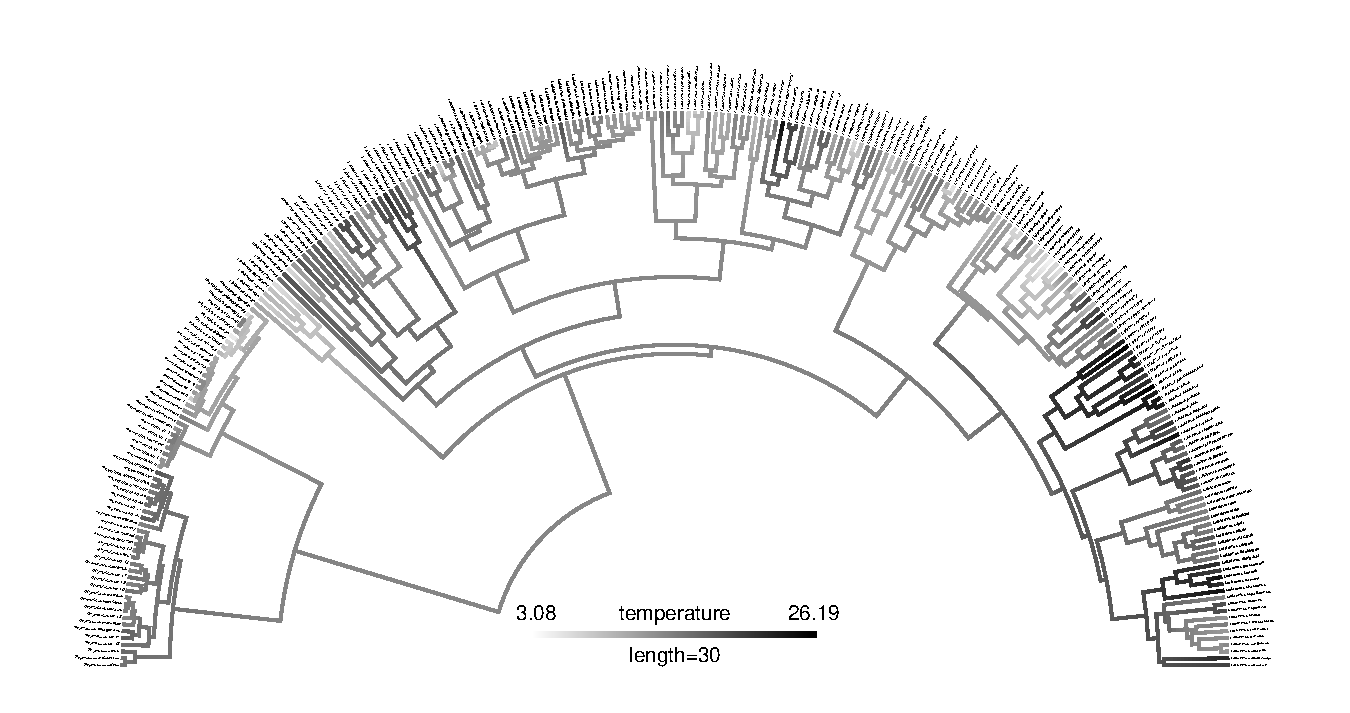
\includegraphics[width=1\linewidth]{Revell.AncestralReconstruction_files/figure-latex/fig11-1} \caption{A phylogenetic tree of the Maximum Likelihood ancestral states (along edges) and observed values (at the tips) of maximum environmental temperature among lizards of the South American family Liolaemidae. The phylogeny and data for this analysis are based on Esquerré et al. (2019). See main text for more details.}\label{fig:fig11}
\end{figure}

\subsubsection{\texorpdfstring{Brownian motion: Body size in the frog genus \emph{Conraua}}{Brownian motion: Body size in the frog genus Conraua}}\label{brownian-motion-body-size-in-the-frog-genus-conraua}

In addition to environmental temperature in Liolaemidae (Figure 11), I also estimated ancestral states for overall body size\footnote{Reported as snout-to-vent length, or SVL (Blackburn et al. 2020).} for African frogs from the genus \emph{Conraua}, known commonly as slippery (Blackburn et al. 2020) or giant (Channing and Rödel 2019) frogs.

The \emph{Conraua} frog clade includes the world's largest frog -- the Goliath frog, \emph{Conraua goliath} -- making their evolutionary history of body size particularly interesting (Blackburn et al. 2020). The tree and data for this example derive from Blackburn et al. (2020) and Channing and Rödel (2019), respectively, and a similar ancestral state reconstruction analysis was undertaken by Blackburn et al. (2020).

To estimate node states in this group, I obtained maximum body size values of six species of \emph{Conraua} frog (Channing and Rödel 2019), along with a single representative value of 53 mm for the outgroup clade Petropedetidae (as in Blackburn et al. 2020), although the latter has been left out of all plots. I transformed all values using the natural logarithm for estimation, and then back-transformed my estimates and their confidence limits to the linear scale for graphing.

Figure 12 shows two different visualizations of ancestral state estimates for \emph{Conraua} frogs. First, Figure panel 12a uses a continuous color gradient (similar to that of Figure 11) mapped to the nodes and tips of the plotted tree. Figure 12b, by contrast, shows a projection of the tree into a phenotype space, called a `traitgram' following Evans et al. (2009; Revell 2013; Revell et al. 2018). Overlain grey polygons give the 95\% confidence intervals around estimated ancestral values. In both graphs, we see the dramatic shift to large body size in the lineage leading to the Goliath frog, \emph{C. goliath} (Figure 12).

\begin{figure}
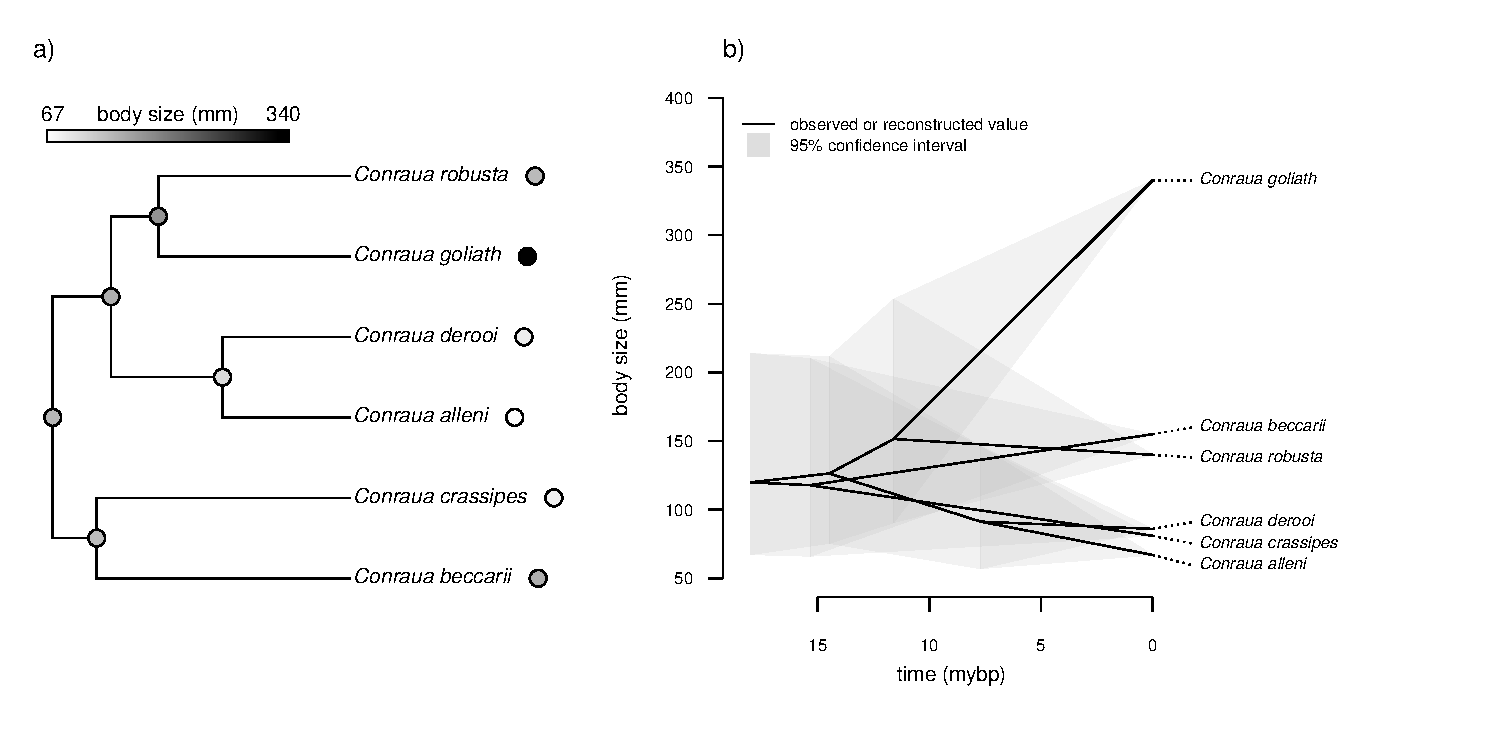
\includegraphics[width=1\linewidth]{Revell.AncestralReconstruction_files/figure-latex/fig12-1} \caption{Ancestral state reconstruction of body size in the \emph{Conraua} frogs. (a) Projection of the observed (at the tips) or estimated (at nodes) ancestral values of body size in mm. (b) Traitgram projection of phylogenetic tree into trait space, based on the ancestral reconstruction. The superimposed grey polygons show 95\% confidence limits around estimated values. The body size data and phylogeny are based on Channing and Rödel (2019) and Blackburn et al. (2020), respectively. See main text for more details.}\label{fig:fig12}
\end{figure}

\section{Properties of ancestral state estimation}\label{properties-of-ancestral-state-estimation}

Though relentlessly popular, ancestral character estimation has been subject to numerous criticisms over the years (e.g., Cunningham et al. 1998; Cunningham 1999; Omland 1999; Losos 2011; Gascuel and Steel 2020). These critiques have assumed (very roughly) two flavors. On the one hand, ancestral state estimates, particularly for nodes close to the root of the tree, tend to have broad uncertainty. Indeed, Ané (2008) shows that the effective sample size\footnote{A measure the amount of independent information contained by the data.} for our estimate of the root node of the tree under Brownian motion tends to be much smaller than the number of tips, and perhaps as small as 5 or 6 for trees containing dozens of terminal taxa, or more (Ané 2008). Similarly, Gascuel and Steel (2020) point out a paradox, or tradeoff, between the conditions under which we can estimate the state at the root of the tree for a discretely-valued trait, and the conditions under which the rates of change between character levels are estimable -- a phenomenon they denominate the `Darwinian uncertainty principle.'\footnote{In short, when the rate of evolution is low, relatively few changes of the trait will have accrued and deep ancestral conditions are straightforward to estimate. On the other hand, these few changes of the trait will have provided little information about the rate of change between character levels. When the rate of change between states is high, on the other hand, precisely the converse will be true. See Gascuel and Steel (2020) for more details.}

Observing that the confidence intervals around ancestral states are broad is not the same as arguing that they are wrong, however: it's merely a reminder that phylogenetic comparative methods are ordinary statistical methods too (Revell et al. 2018; Revell and Harmon 2022). As such, it would be incorrect to treat an estimated ancestral state as if it were a quantity known without error (Losos 2011). Indeed, when the our underlying model assumptions are valid, ancestral state estimation has suitable statistical properties (Revell and Harmon 2022).

A more pernicious problem arises when the model is wrong (Revell and Harmon 2022).\footnote{Or, rather `badly wrong' -- seeing how, in point of fact, all models are wrong, even if many are useful (to paraphrase the statistician George Box, 1976).} Under these circumstances, it becomes possible to \emph{confidently} estimate wrong ancestral node states.\footnote{This, too, one could argue, falls into the category of ancestral state reconstruction behaving as do all normal statistical methods! On the other hand, some evidence suggests that ancestral reconstruction is particularly sensitive to model assumption violations.}

To investigate ancestral state estimation when model assumptions are violated, I'll consider three different case studies: discrete character evolution under the hidden-rates model (Beaulieu et al. 2013); discrete trait evolution under the threshold model (Felsenstein 2005, 2012; Revell 2014a); and bounded Brownian evolution (Boucher and Démery 2016). I'll show that when an incorrect model is used (specifically, a homogenous-rate M\emph{k} model for the discrete data and unbounded Brownian motion for continuous characters), bad statistical behavior emerges. On the other hand, however, I will also show that this effect is substantively diminished under the correct, generating model for each case.

\subsection{Ancestral state estimation when the model is right}\label{ancestral-state-estimation-when-the-model-is-right}

Before showing that ancestral state estimation can misbehave when the model of evolution is \emph{wrong}, it seems useful to undertake a very brief exploration of the properties of ancestral state reconstruction when the model used for estimation fully captures the generating evolutionary process: in other words, when the model is ``right.'' This is genuinely the best case scenario for ancestral character estimation, so we might expect to find statistical properties are optimal in this scenario.

To begin with, I simulated 100 stochastic, pure-birth phylogenies, each containing a total of 501 taxa (and thus 500 internal nodes), with a total root to tip height of 10.0.\footnote{This tree depth has no particular meaning. By trial and error I discovered that it tended to result in a relatively even distribution of marginal scaled likelihoods across simulations.} I next generated one binary (0/1) character and one continuous character for each tree. The discrete character was simulated with a generating value of \textbf{Q} that matched the illustrative value of \textbf{Q} used earlier in the article.

\[\mathbf{Q} = \begin{bmatrix}-q_{0,1} & q_{0,1} \\ q_{1,0} & -q_{1,0}\end{bmatrix} = \begin{bmatrix}-0.2 & 0.2\\ 0.2 & -0.2\end{bmatrix}\]

In addition to this discretely-valued character, I also simulated one continuous trait for each tree under Brownian motion using a starting value of \(x_0 = 0.0\) and a Brownian motion (stochastic diffusion) rate of \(\sigma^2 = 1.0\).

\begin{figure}
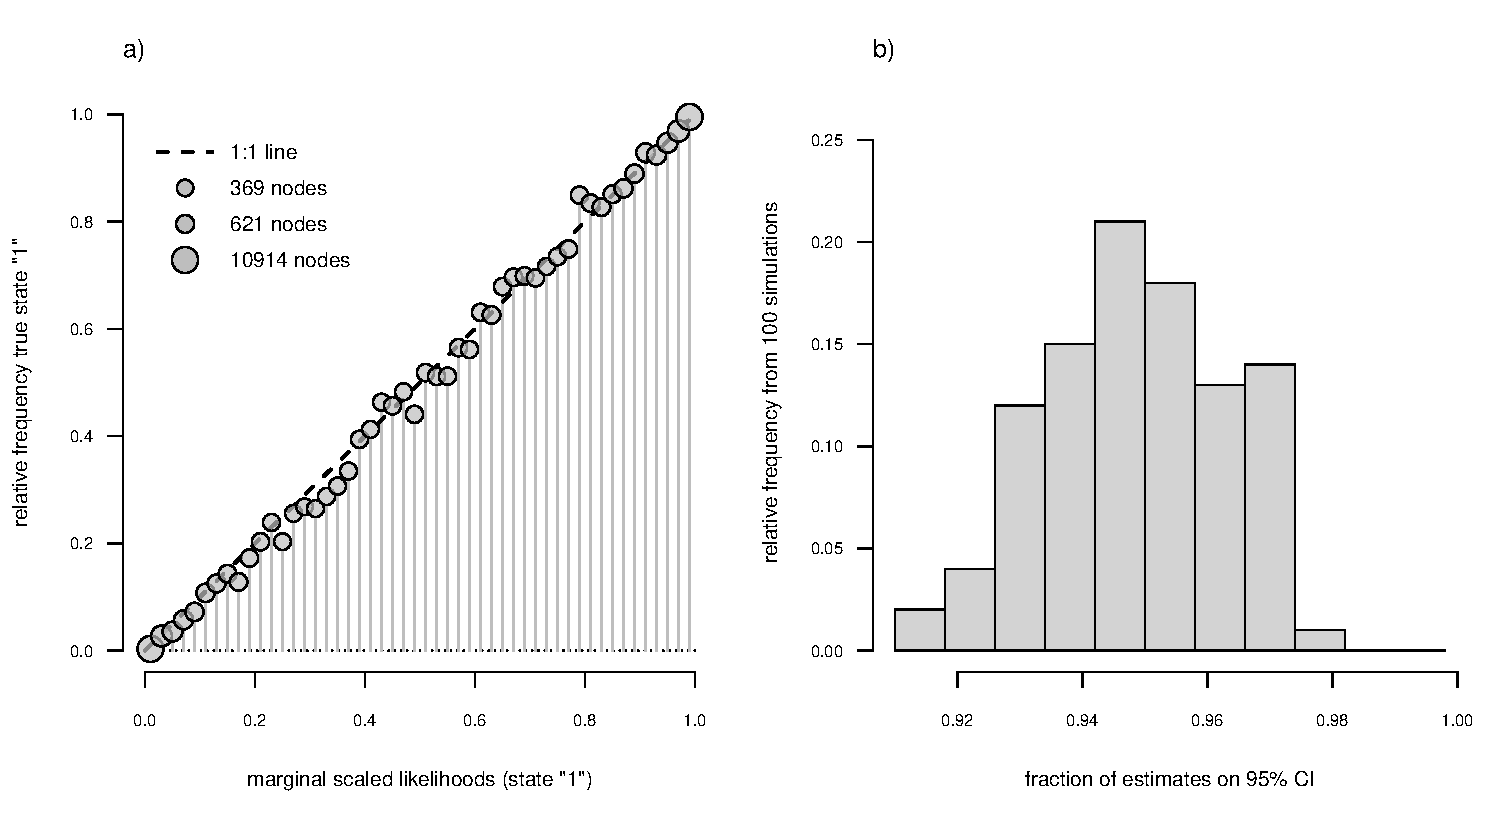
\includegraphics[width=1\linewidth]{Revell.AncestralReconstruction_files/figure-latex/fig13-1} \caption{Accuracy of ancestral state reconstruction of discrete (a) and continuous (b) characters when the model for estimation is correct. (a) Node marginal scaled likelihoods (of state ``1'') compared to the relative frequency that each node was in that condition. If the scaled likelihoods are an accurate measure of the true probability of that each node was in each character state, then these values should form a 1:1 line. Point diameters have been scaled by the natural logarithm of the sample size (number of nodes) for each bin. (b) Distribution of the relative frequency (from 100 simulations) in which the true ancestral value fell on the 95\% confidence interval of each node estimate, averaged across all nodes by simulation. See main text for additional details.}\label{fig:fig13}
\end{figure}

To measure the performance of ancestral state reconstruction for discrete characters when the generating model was known and used for estimation, I first binned the marginal scaled likelihoods of the node being in condition ``1'' into 50 equal-sized intervals, each 0.02 units wide. For each bin, I then simply counted the number of nodes across all simulations whose true states were equal to ``1''. This count, divided by the \emph{total} number of nodes in that bin, would be expected to be equal to the midpoint of the bin if the marginal scaled likelihoods genuinely correspond to a probability that the node is in each state, under the model. So, for instance, if the marginal scaled likelihood ban spanned 0.19 through 0.21, with a midpoint of 0.2, then we would expect to find that (on average) 20\% of nodes in this bin should be in condition ``1'' (and 80\% thus in condition ``0''), and so on.\footnote{If I'm not mistaken, B. O'Meara originally suggested this to me as a procedure for measuring the accuracy of a statistical method designed to compute probabilities during the \emph{Evolution} conference some years ago now.}

To measure the performance of ancestral state estimation when the generating model was known for continuous characters, I simply quantified the fraction of node-wise 95\% confidence intervals for which the true value fell within the interval.\footnote{I could have also measured the correlation between the generating and estimated values, or the average difference (bias) between the known values and the estimates.}

Figure 13 summarizes the results of this analysis. In Figure 13a, we see that the relative frequency of being in condition ``1'' closely tracks the marginal scaled likelihoods. In Figure 13b, we likewise see that the distribution of true node values that fall on the 95\%, averaged by simulation, is centered closely on 95\%, with a mean of 94.98\% and a range of \([0.916, 0.976]\) (Figure 13). In summary, when the model for estimation is \emph{correct}, ancestral state reconstruction can work precisely as intended.

\subsection{Ancestral state estimation when the model is wrong}\label{ancestral-state-estimation-when-the-model-is-wrong}

In the previous section, I illustrated how ancestral state reconstruction can be statistically well-behaved when the model for estimation is correct. Using a trio of very simple examples, I'll now try to demonstrate how ancestral character estimation might go astray when the model for estimation is badly wrong. I'll do this by simulating data under three different trait evolution models that we haven't yet discussed: two for discrete characters; and a third for continuous traits. Note that the purpose of this section is not to prove that we can recover the good statistical behavior of ancestral state reconstruction when the \emph{correct} model is used, though that is sometimes true and will be true in these particular cases. To the contrary, my intention is to highlight the substantial sensitivity or vulnerability to model assumption violations of our standard reconstruction methods.

\subsubsection{Ancestral states under a hidden-rates model}\label{ancestral-states-under-a-hidden-rates-model}

To show this, I'll first use a model called the hidden-rates model (Marazzi et al. 2012; Beaulieu et al. 2013; Boyko and Beaulieu 2021; Revell and Harmon 2022; Revell 2024). The hidden-rates model is one in which, for each observed level of a discrete trait, there might be one or more unobserved conditions, each with their own rates of transition of the observed state. Figure 14 illustrates evolution under a flavor of the hidden-rates model in which the observed condition ``1'' has two hidden levels: ``1'' in which the trait can still transition back to the ``0'' form; and ``1*'' in which it cannot.\footnote{The character codndition of ``1*'' is also then an `absorbing' state for the character.} An attribute of trait evolution under the hidden-rates model is heterogeneity in the rate of transition between states. This is apparent in Figure 14b and 14c in which we see that transitions occur frequently between the two visible conditions of the trait, ``0'' and ``1'', until the condition ``1'' changes to the hidden state ``1*'' (Figure 14). It's relatively easy to imagine a trait that could evolve in this way. Considering parity mode in squamate reptiles, for instance, perhaps when viviparity (which, in some squamates might be called `ovoviviparity' and is little more than egg retention through hatching), has recently evolved, it can still be lost. Over time, however, additional adaptations or loss of function mutations accumulate and viviparity eventually evolves into a condition from which oviparity can no longer re-emerge. This evolutionary scenario would be well-captured by the model illustrated in Figure 14.

\begin{figure}
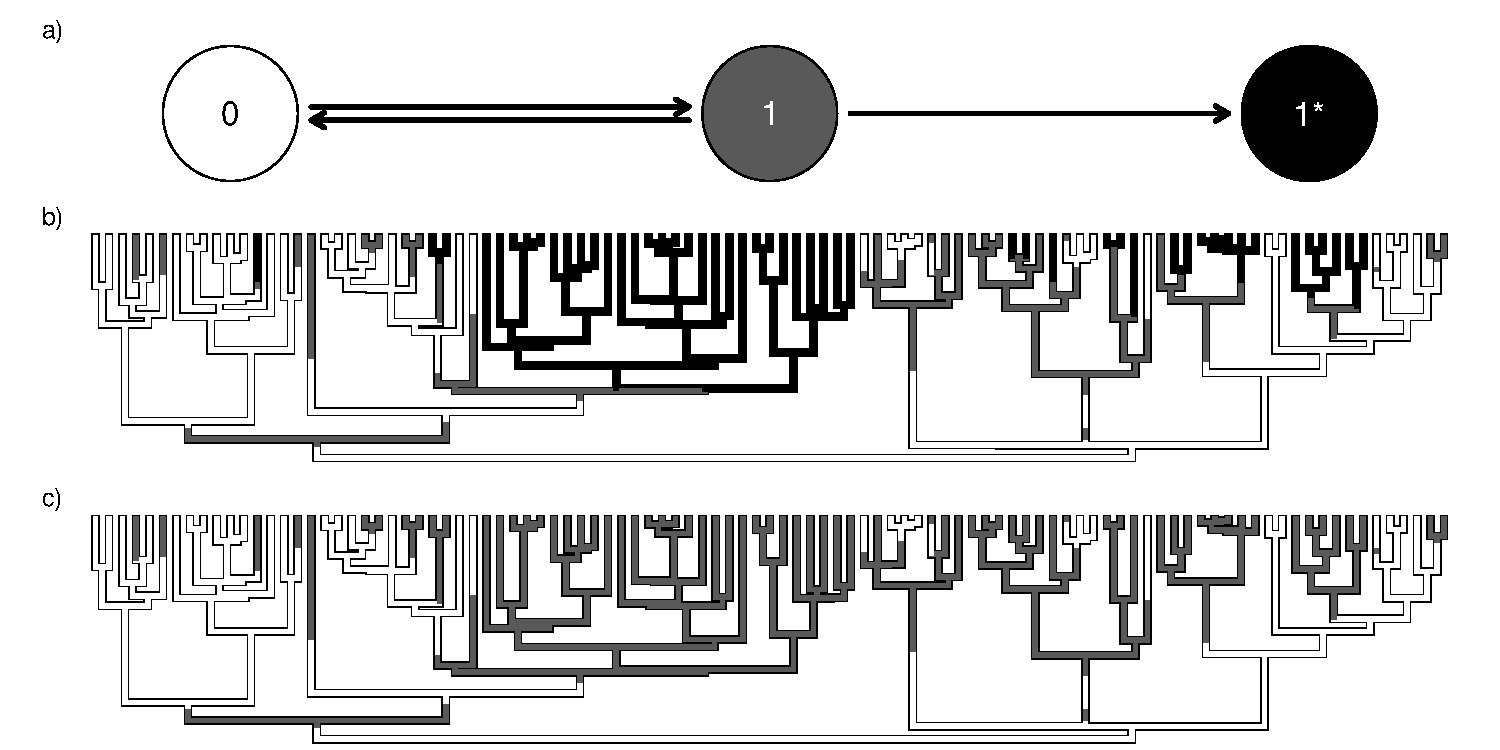
\includegraphics[width=1\linewidth]{Revell.AncestralReconstruction_files/figure-latex/fig14-1} \caption{A graphical illustration of the hidden rates model. (a) The structure of a hidden-rates model with one hidden, absorbing condition (``1*'') of the observed level ``1''. (b) Simulated evolution with both hidden levels of ``1'' shown. (c) Simulated history from (b), but with the two levels of ``1'' merged into a single, observed trait. See main text for more details.}\label{fig:fig14}
\end{figure}

To simulate under this model I used the following transition matrix, \textbf{Q}, between observed and unobserved levels of each of the two trait conditions.

\[
\mathbf{Q} = 
\begin{bNiceMatrix}[first-row,first-col]
& 0 & 1 & 1* \\
0 & -0.20 & 0.20 & 0.00 \\
1 & 0.20 & -0.30 & 0.10 \\
1* & 0.00 & 0.00 & 0.00
\end{bNiceMatrix}
\]

I used the same one hundred, 501 taxon phylogenies that were simulated for the previous section. After simulation, I merged the two different hidden levels of character ``1'' (that is, ``1'' and ``1*'') into a single, observed character condition.\footnote{This is because in empirical studies the `hidden' level of character ``1'' and its unhidden condition are the same observed state!} Finally, as opposed to estimating ancestral states under the correct model, I began by using an incorrect model of evolution without hidden states, but in which the back-and-forth transition rates between the two observed character conditions were allowed to occur with different rhythms.

\begin{figure}
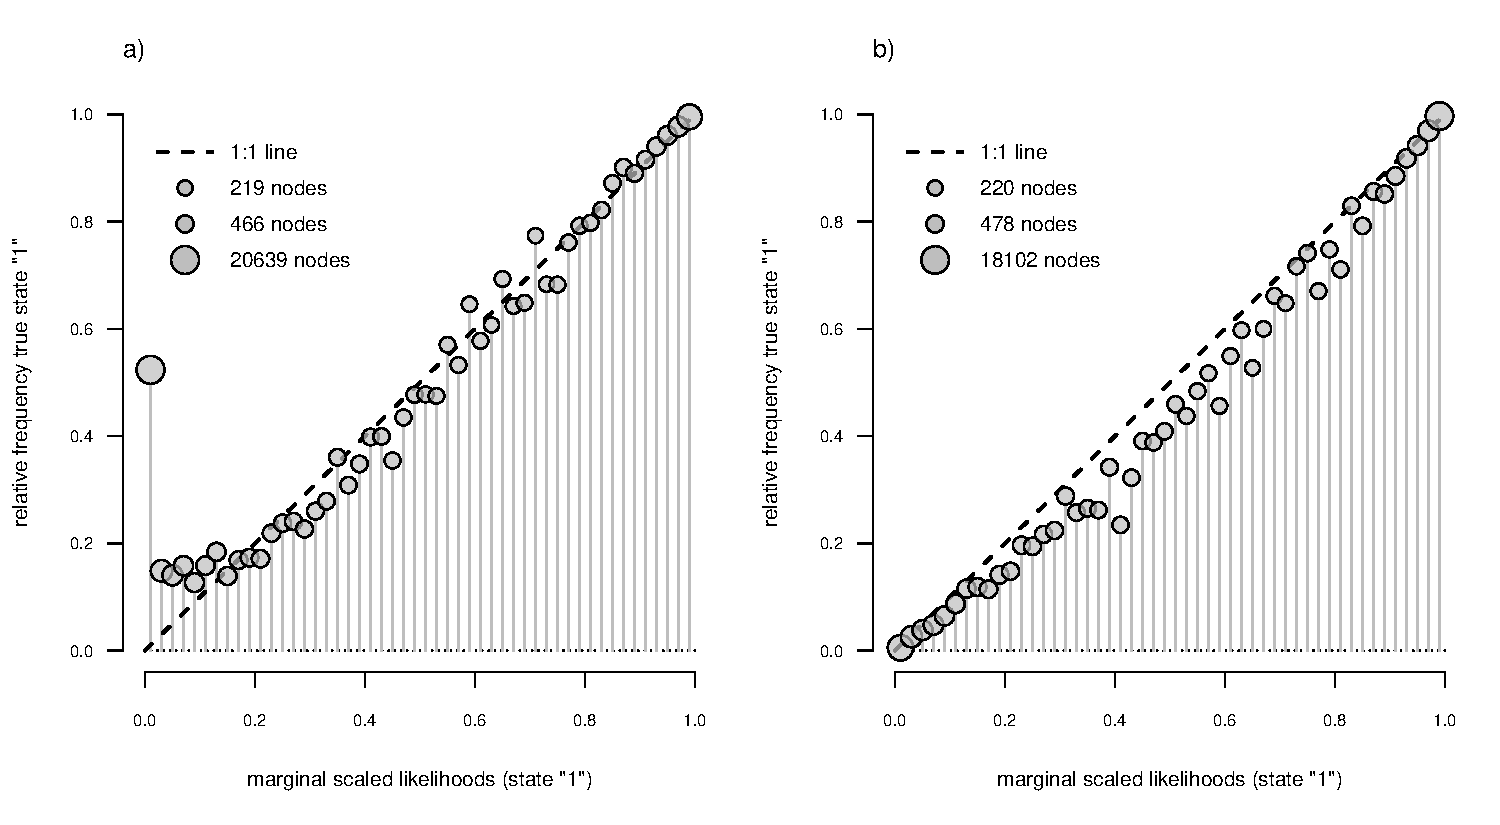
\includegraphics[width=1\linewidth]{Revell.AncestralReconstruction_files/figure-latex/fig15-1} \caption{Accuracy of ancestral state reconstruction of discrete characters when the hidden rate model of Figure 14 was used for simulation. (a) Node marginal scaled likelihoods (of state ``1'') compared to the relative frequency that each node was in that condition using a standard M\emph{k} model for estimation. (b) The same as (a), but in which the generating hidden-rates model was used. If the scaled likelihoods are an accurate measure of the true probability of that each node was in each character state, then these values should form a 1:1 line. As in Figure 13, point diameters have been scaled by the natural logarithm of the sample size (number of nodes) for each bin.  See main text for additional details.}\label{fig:fig15}
\end{figure}

The result from this analysis is given in Figure 15a. Even though most points fall on the 1:1 line, we also see a large fraction of nodes that are not resolved into one condition or the other, even though they have (known) true state ``0'' (Figure 15a).

In addition to simply reconstructing under the standard M\emph{k} model, we also fit and estimated ancestral states using the hidden-rates model, which was the generating evolutionary scenario of our data. The results from this analysis are given in Figue 15b which more closely resembles panel a of Figure 13 (in which the true model was known and used for estimation) than it does Figure 15a. This suggests that good statistical properties of estimation are largely recovered when the correct model is used.

\subsection{Ancestral states under the threshold model}\label{ancestral-states-under-the-threshold-model}

The next discrete character evolution model that we'll consider is one that's called the threshold model (Wright 1934; Felsenstein 2005, 2012). Under the threshold model, our discrete character is underlain by an unobserved quantitative trait called `liability.' Every time liability crosses a pre-defined (but unknown) threshold, our observed discrete character changes state. The model derives originally from evolutionary quantitative genetics where it was used by Wright (1934) to describe variation in digit number of guinea pigs, but was much later adapted by Felsenstein (2005; 2012) to phylogenetic comparative biology. A simulation of discrete character evolution under the threshold model is given in Figure 16. Panel (a) of the figure shows the Brownian evolution of the normally unobserved liabilities (and thresholds), whereas panel (b) illustrates the resultant discrete trait evolution on the branches and nodes of the phylogeny.

\begin{figure}
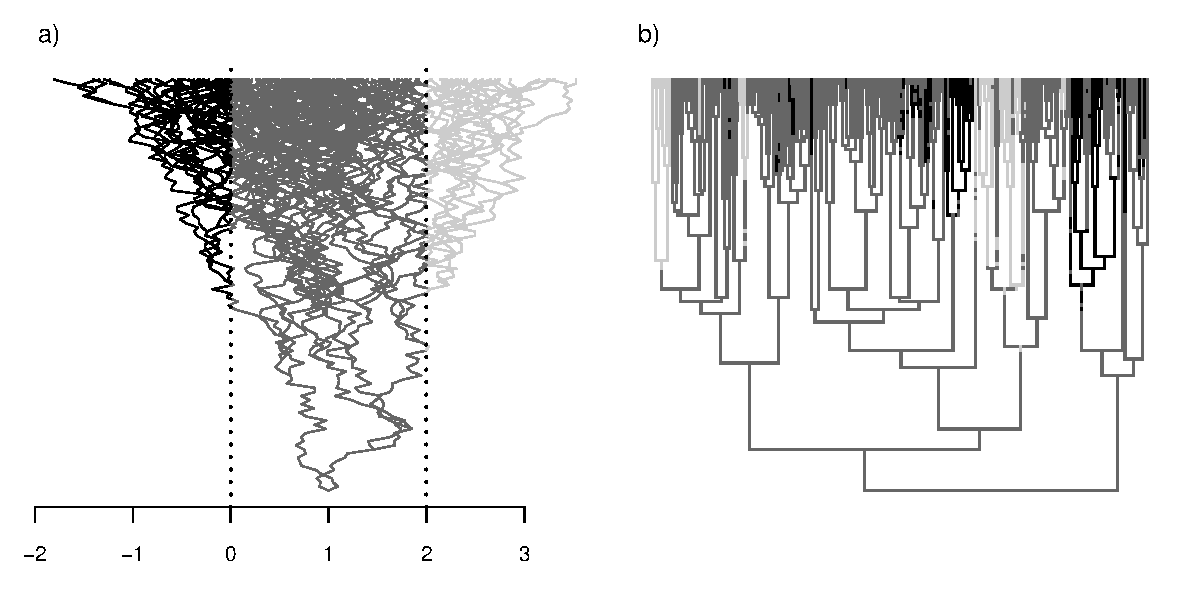
\includegraphics[width=1\linewidth]{Revell.AncestralReconstruction_files/figure-latex/fig16-1} \caption{Illustration of evolution under the threshold model. (a) The evolution of liabilities: the unobserved continuous character whose condition determines the state of the discrete trait. The thresholds between discrete character levels in the threshold trait are shown using the vertical dotted lines. (b) The realized evolution of the discrete character across the branches and nodes of the phylogeny. See main text for more details.}\label{fig:fig16}
\end{figure}

Various features of the evolution of our discrete character are manifestly different between Figure 16b and evolution under a standard M\emph{k} scenario. Most conspicuously, and not unlike the hidden-rates model of Figure 14, the tempo of evolutionary change for the discrete trait varies from clade to clade of the tree. This is because in parts of the tree where the evolutionary process for the liability is close to a threshold, the character changes frequently in state. By contrast, when the liability is far from any threshold, the discrete character may experience long periods of stasis with little to no change at all (Revell 2014a; Revell and Harmon 2022).

To simulate evolution under the threshold model, I used the same one hundred, 501 taxon phylogenies that were simulated for the previous sections. I next simulated a continuous trait (liability) evolving via Brownian motion with a rate equal to \(\sigma^2 = 0.1\), an ancestral value of \(x_0 = 2.0\), and thresholds between character levels of \([0, 1, 3]\).\footnote{This typically resulted in four levels of the discrete character, but in a small subset of simulations only three character levels were observed.} For each dataset, I fit an ordered M\emph{k} model,\footnote{I chose to do this because the threshold model itself is intrinsically ordered.} as well as the threshold model. To fit the threshold model I used the discrete approximation of Boucher and Démery (2016; Revell 2024). For each fitted model, I computed marginal ancestral states in the typical way. Finally, as in Figure 16, I compared the marginal scaled likelihoods that each node was in each state to the \emph{genuine} frequency of the node being in the corresponding condition. If the ancestral state reconstruction method is working properly, these values should form a 1:1 line. The result of this analysis is shown in Figure 17.

\begin{figure}
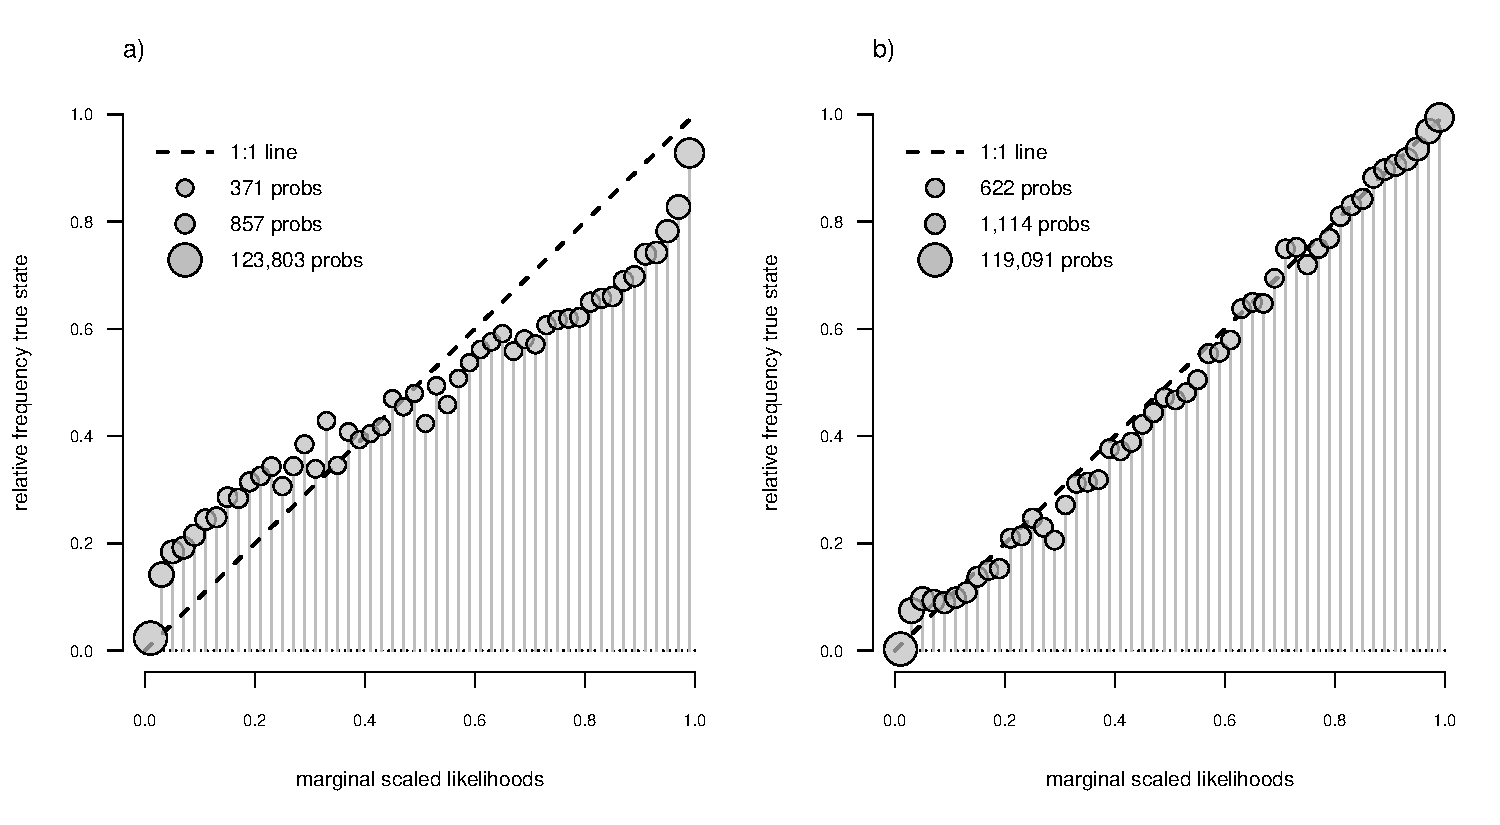
\includegraphics[width=1\linewidth]{Revell.AncestralReconstruction_files/figure-latex/fig17-1} \caption{Accuracy of ancestral state reconstruction of discrete characters when the threshold model of Figure 16 was used for simulation. (a) Node marginal scaled likelihoods compared to the relative frequency that each node was in that condition using a standard M\emph{k} model for estimation. (b) The same as (a), but in which the generating threshold model was used for estimation. If the scaled likelihoods are an accurate measure of the true probability of that each node was in each character state, then these values should form a 1:1 line. Point diameters have been scaled by the natural logarithm of the sample size (total number of probabilities computed) for each bin. Note that these don't sum to the number of nodes because multiple values are calculated for each node in each simulation, depending on the number of levels (3 or 4) of the trait. See main text for additional details.}\label{fig:fig17}
\end{figure}

As is evident from the figure, I found marginal ancestral reconstruction to be quite inaccurate when the M\emph{k} model was used for estimation (Figure 17a). In particular, marginal scaled likelihoods tended to overestimate the probability that a node was in each state when low, and underestimate the same quantity when high (Figure 17a). In contrast, when estimation was performed using the generating, threshold model, good statistical behavior of marginal estimation was fully recovered (Figure 17b).

\subsubsection{Ancestral states under bounded Brownian motion}\label{ancestral-states-under-bounded-brownian-motion}

As discussed earlier in this article, the typical model for ancestral state reconstruction of continuous traits is one of unbounded Brownian motion evolution, also known as stochastic diffusion or a continuous time random walk. To investigate the sensitivity of continuous character ancestral state reconstruction to model misspecification, we first generated 100 datasets, one for each our 100 simulated 501 taxon trees of the previous two sections. In this case, however, our generating model is \emph{bounded} Brownian evolutionary change, with \(x_0 = 0.0\), \(\sigma^2 = 1.0\), and upper and lower bounds of \([-2, 2]\). Bounded Brownian motion (with reflective bounds) is just like standard Brownian motion, but in which whenever the boundary condition is reached, the evolutionary process reflects back into the bounded space (Boucher and Démery 2016).

Following simulation, we first reconstructed ancestral states under a standard (unbounded) Brownian model, and then under \emph{bounded} Brownian evolution, the latter utilizing the method of Boucher and Démery (2016). We measured the statistical behavior of ancestral state estimation in the same way as in Figure 13b; however, since the true value of an estimated parameter might fall within the confidence interval of the estimate either because the estimate is accurate or because the confidence interval is wide, we \emph{also} measured accuracy of ancestral estimates by calculating the correlation between the known generating values and the estimates for each simulation. The results of this analysis are given in Figure 18.

\begin{figure}
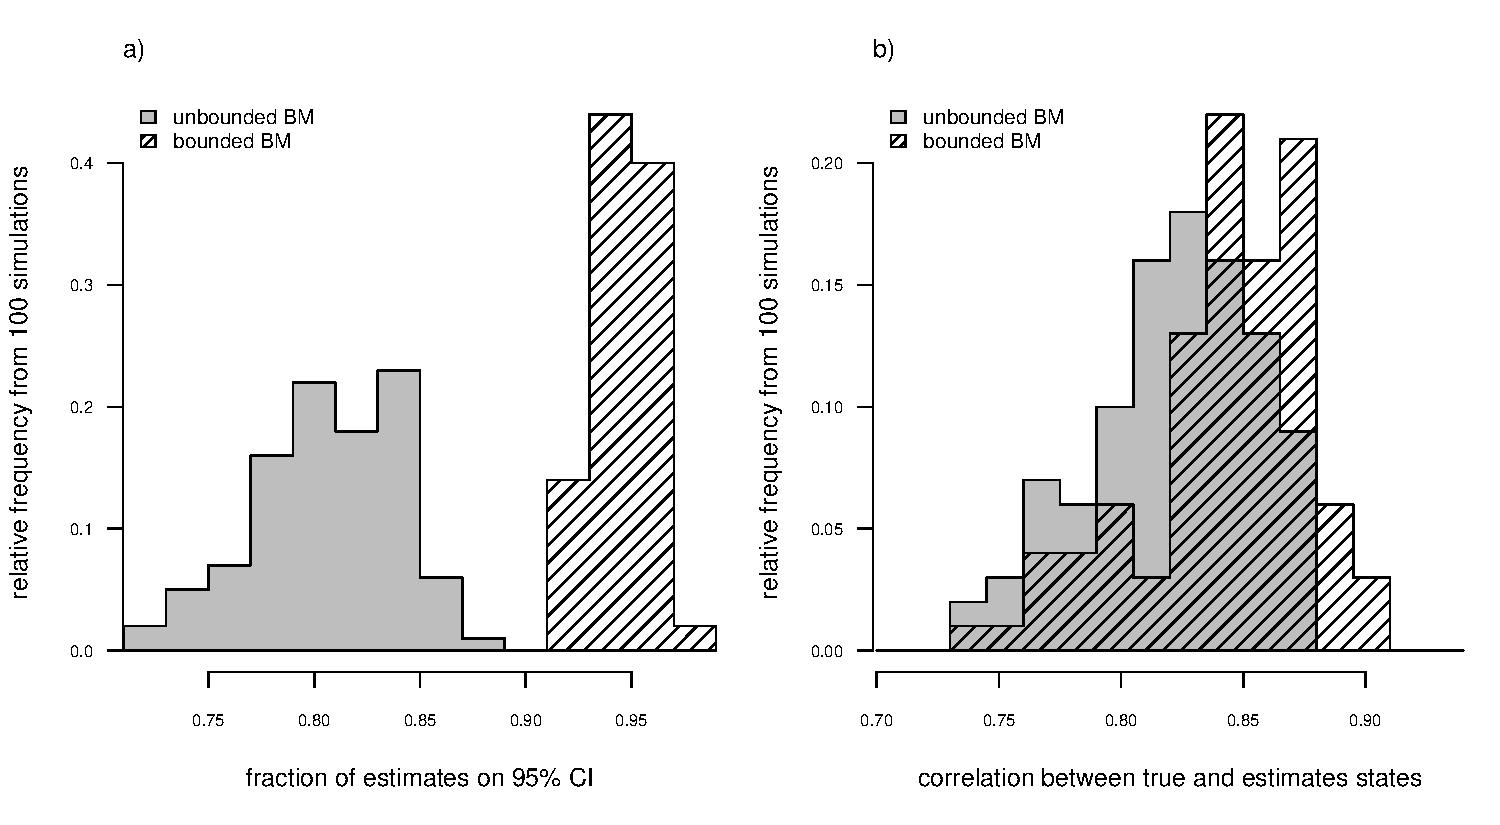
\includegraphics[width=1\linewidth]{Revell.AncestralReconstruction_files/figure-latex/fig18-1} \caption{Accuracy of ancestral state reconstruction of  continuous characters when data were simulated under Brownian motion evolution with reflective bounds. (a) Frequency distribution of the fraction of nodes falling in within the 95\% confidence interval of each node estimate, averaged across all nodes by simulation both when a standard Brownian model (grey) and bounded model (shading lines) was used for estimation. (b) Distribution of correlation between true and estimated ancestral states when the data were generated under bounded Brownian evolution, and either a standard Brownian motion model (grey) or bounded model (shading lines) was used for estimation. See main text for additional details.}\label{fig:fig18}
\end{figure}

We see that when data are simulated under bounded Brownian evolution, but unbounded Brownian motion is assumed as a model for estimation, confidence intervals are too narrow (Figure 18a), with a mean fraction of true ancestral states falling within the 95\% confidence intervals of the estimates of 80.8\% (range: \([71.6, 87.6]\); Figure 18a). By contrast, almost exactly 95\% of confidence intervals estimated under \emph{bounded} Brownian evolution (Boucher and Démery 2016) included the true, generating values of the states (average: 94.6\%; range: \([92.0, 97.8]\); Figure 16a).

In addition to having the correct confidence intervals, estimates obtained under bounded Brownian motion were also more accurate (Figure 18b). The mean correlation between generating and estimated ancestral states when \emph{unbounded} Brownian evolution was assumed as a model for estimation was \(\bar{r} = 0.822\) -- compared to a mean of \(\bar{r} = 0.843\) when the correct model was used (Figure 18b).

\section{Software implementation and data availability}\label{software-implementation-and-data-availability}

Ancestral character estimation is implemented in the R statistical computing software (R Core Team 2024) package \emph{phytools} (Revell 2012, 2024), as well as in a number of other R packages and software (e.g., Schliep 2011; Paradis and Schliep 2019; Boyko and Beaulieu 2021; Beaulieu et al. 2023; Maddison and Maddison 2023; Pagel and Meade 2024). All analyses of this article were conducted using \emph{phytools}. \emph{phytools} in turn depends on the core R phylogenetics packages \emph{ape} (Paradis and Schliep 2019) and \emph{phangorn} (Schliep 2011). \emph{phytools}, \emph{ape}, and \emph{phangorn} are all publicly available through the Comprehensive R Archive Network, CRAN (\url{https://cran.r-project.org/}). All data and code of this article can be reviewed via the public GitHub repository, \url{https://github.com/liamrevell/Revell.AncestralReconstruction}.

\section{Conclusions}\label{conclusions}

Ancestral state reconstruction has long been among the most relentlessly popular analyses of phylogenetic comparative biology. In this article, I have tried to overview the theoretical and practical basics of ancestral state reconstruction for discrete and continuously-valued character traits. I have shown how ancestral state reconstruction can be applied to empirical datasets of various types, such as estimating the ancestral conditions of environmental temperature in liolaemid lizards, diel activity pattern in primates, or body size in frogs.

In spite of its popularity, ancestral state estimation has some limitations. In particular, ancestral node estimates often come associated with very broad confidence limits, deep in the phylogenetic tree. Additionally, ancestral state reconstruction can be highly sensitive to violations of the assumptions of the evolutionary model used for estimation. Though both of these attributes (broad confidence intervals when the amount of information about a parameter is low; and sensitivity to model assumptions) are properties of many statistical inference methods, enthusiasts of ancestral state reconstruction have sometimes failed to sufficiently appreciate the nature and depth of these limitations.

In an age when phylogenetic data is ever easier to produce, I have little doubt that the appeal of ancestral character state reconstruction will continue to grow into the future. I hope that this article will provide a helpful introductory guide to those biologists and scientists of other disciplines who dare to venture into this endeavor.

\section{A short postscript on the origins of this article}\label{a-short-postscript-on-the-origins-of-this-article}

Some time during 2023 I was asked to contribute a section on `Ancestral Reconstruction: Theory \& Practice' for the second edition of a compendium titled the `Encyclopedia of Evolutionary Biology' (Kliman 2016). Not having carefully read the instructions, but enthusiastic about the task, I proceeded to write what I expected to be a lengthy book chapter on the subject, including some original primary research on the accuracy of ancestral state reconstruction under different circumstances. As it turns out, and as I realized before submitting my article to the publisher, this was totally inconsistent with the aims of the project which called for a much more compact and less detailed treatment of the subject. Having identified my blunder, I was forced to go back to the drawing board and produce a much more appropriate length piece for the encyclopedia. The present article is the fruit of my original labor and is geared towards researchers more interested in the technical details of ancestral reconstruction and its application.\footnote{As a sidenote, here recorded unironically as a footnote, let me add that though they overlap thematically, all of the text and content of this article is original and not redundant with my \emph{Encyclopedia of Evolutionary Biology} entry!} I hope that it can serve this purpose here.

\section*{References}\label{references}
\addcontentsline{toc}{section}{References}

\phantomsection\label{refs}
\begin{CSLReferences}{1}{0}
\bibitem[\citeproctext]{ref-Anderson2017}
Anderson, S. R., and J. J. Wiens. 2017. \href{https://doi.org/10.1111/evo.13284}{Out of the dark: 350 million years of conservatism and evolution in diel activity patterns in vertebrates: Evolution of day-night activity patterns}. Evolution 71:1944--1959. Wiley.

\bibitem[\citeproctext]{ref-Ane2008}
Ané, C. 2008. \href{https://doi.org/10.1214/08-aoas173}{Analysis of comparative data with hierarchical autocorrelation}. The Annals of Applied Statistics 2. Institute of Mathematical Statistics.

\bibitem[\citeproctext]{ref-Baum2012-book}
Baum, D. A., and S. D. Smith. 2012. Tree thinking: An introduction to phylogenetic biology. W.H. Freeman, New York, NY.

\bibitem[\citeproctext]{ref-Beaulieu2013}
Beaulieu, J. M., B. C. O'Meara, and M. J. Donoghue. 2013. \href{https://doi.org/10.1093/sysbio/syt034}{Identifying hidden rate changes in the evolution of a binary morphological character: The evolution of plant habit in campanulid angiosperms}. Systematic Biology 62:725--737. Oxford University Press (OUP).

\bibitem[\citeproctext]{ref-Beaulieu2023}
Beaulieu, J., B. O'Meara, J. Oliver, and J. Boyko. 2023. \href{https://github.com/thej022214/corHMM}{corHMM: Hidden markov models of character evolution}.

\bibitem[\citeproctext]{ref-BetancurR2015}
Betancur‐R., R., G. Ortí, and R. A. Pyron. 2015. \href{https://doi.org/10.1111/ele.12423}{Fossil‐based comparative analyses reveal ancient marine ancestry erased by extinction in ray‐finned fishes}. Ecology Letters 18:441--450. Wiley.

\bibitem[\citeproctext]{ref-Blackburn2020}
Blackburn, D. C., S. V. Nielsen, M. F. Barej, J. Doumbia, M. Hirschfeld, N. G. Kouamé, D. Lawson, S. Loader, C. Ofori‐Boateng, E. L. Stanley, and M. Rödel. 2020. \href{https://doi.org/10.1111/zsc.12447}{Evolution of the {A}frican slippery frogs ({A}nura: {C}onraua), including the world's largest living frog}. Zoologica Scripta 49:684--696. Wiley.

\bibitem[\citeproctext]{ref-Blomberg2003}
Blomberg, S. P., T. Garland, and A. R. Ives. 2003. \href{https://doi.org/10.1111/j.0014-3820.2003.tb00285.x}{Testing for phylogenetic signal in comparative data: Behavioral traits are more labile}. Evolution 57:717--745. Wiley.

\bibitem[\citeproctext]{ref-Bollback2006}
Bollback, J. P. 2006. \href{https://doi.org/10.1186/1471-2105-7-88}{{SIMMAP}: Stochastic character mapping of discrete traits on phylogenies}. BMC Bioinformatics 7. Springer Science; Business Media LLC.

\bibitem[\citeproctext]{ref-Boucher2016}
Boucher, F. C., and V. Démery. 2016. \href{https://doi.org/10.1093/sysbio/syw015}{Inferring bounded evolution in phenotypic characters from phylogenetic comparative data}. Systematic Biology 65:651--661. Oxford University Press (OUP).

\bibitem[\citeproctext]{ref-Box1976}
Box, G. E. P. 1976. \href{https://doi.org/10.1080/01621459.1976.10480949}{Science and statistics}. Journal of the American Statistical Association 71:791--799. Informa UK Limited.

\bibitem[\citeproctext]{ref-Boyko2021}
Boyko, J. D., and J. M. Beaulieu. 2021. \href{https://doi.org/10.1111/2041-210x.13534}{Generalized hidden markov models for phylogenetic comparative datasets}. Methods in Ecology and Evolution 12:468--478. Wiley.

\bibitem[\citeproctext]{ref-Channing2019}
Channing, A., and M.-O. Rödel. 2019. Field guide to frogs and other amphibians of {A}frica. Struik Nature, Cape Town, South Africa.

\bibitem[\citeproctext]{ref-Churchill2021}
Churchill, M., and C. Baltz. 2021. \href{https://doi.org/10.1111/joa.13522}{Evolution of orbit size in toothed whales ({A}rtiodactyla: {O}dontoceti)}. Journal of Anatomy 239:1419--1437. Wiley.

\bibitem[\citeproctext]{ref-Cunningham1999}
Cunningham, C. W. 1999. \href{https://doi.org/10.1080/106351599260238}{Some limitations of ancestral character-state reconstruction when testing evolutionary hypotheses}. Systematic Biology 48:665--674. Oxford University Press (OUP).

\bibitem[\citeproctext]{ref-Cunningham1998}
Cunningham, C. W., K. E. Omland, and T. H. Oakley. 1998. \href{https://doi.org/10.1016/s0169-5347(98)01382-2}{Reconstructing ancestral character states: A critical reappraisal}. Trends in Ecology and Evolution 13:361--366. Elsevier BV.

\bibitem[\citeproctext]{ref-Danis2023}
Danis, T., and A. Rokas. 2023. The evolution of gestation length in eutherian mammals.

\bibitem[\citeproctext]{ref-DurnCastillo2021}
Durán‐Castillo, M., A. Hudson, Y. Wilson, D. L. Field, and A. D. Twyford. 2021. \href{https://doi.org/10.1111/nph.17581}{A phylogeny of {A}ntirrhinum reveals parallel evolution of alpine morphology}. New Phytologist 233:1426--1439. Wiley.

\bibitem[\citeproctext]{ref-Esquerr2019}
Esquerré, D., I. G. Brennan, R. A. Catullo, F. Torres‐Pérez, and J. S. Keogh. 2019. \href{https://doi.org/10.1111/evo.13657}{How mountains shape biodiversity: The role of the andes in biogeography, diversification, and reproductive biology in {S}outh {A}merica's most species‐rich lizard radiation ({S}quamata: {L}iolaemidae)}. Evolution 73:214--230. Wiley.

\bibitem[\citeproctext]{ref-Evans2009}
Evans, M. E. K., S. A. Smith, R. S. Flynn, and M. J. Donoghue. 2009. \href{https://doi.org/10.1086/595757}{Climate, niche evolution, and diversification of the {``bird‐cage''} evening primroses ({O}enothera, sections {A}nogra and {K}leinia)}. The American Naturalist 173:225--240. University of Chicago Press.

\bibitem[\citeproctext]{ref-Faurby2016}
Faurby, S., W. L. Eiserhardt, W. J. Baker, and J.-C. Svenning. 2016. \href{https://doi.org/10.1016/j.ympev.2016.03.002}{An all-evidence species-level supertree for the palms ({A}recaceae)}. Molecular Phylogenetics and Evolution 100:57--69. Elsevier BV.

\bibitem[\citeproctext]{ref-Felsenstein2012}
Felsenstein, J. 2012. \href{https://doi.org/10.1086/663681}{A comparative method for both discrete and continuous characters using the threshold model}. The American Naturalist 179:145--156. University of Chicago Press.

\bibitem[\citeproctext]{ref-Felsenstein1981}
Felsenstein, J. 1981. \href{https://doi.org/10.1007/bf01734359}{Evolutionary trees from DNA sequences: A maximum likelihood approach}. Journal of Molecular Evolution 17:368--376. Springer Science; Business Media LLC.

\bibitem[\citeproctext]{ref-Felsenstein2004-book}
Felsenstein, J. 2004. Inferring phylogenies. Sinauer associates, Sunderland, MA.

\bibitem[\citeproctext]{ref-Felsenstein1973-a}
Felsenstein, J. 1973. Maximum-likelihood estimation of evolutionary trees from continuous characters. American Journal of Human Genetics 25:471--492.

\bibitem[\citeproctext]{ref-Felsenstein1985}
Felsenstein, J. 1985. Phylogenies and the comparative method. Am. Nat. 125:1--15.

\bibitem[\citeproctext]{ref-Felsenstein2005}
Felsenstein, J. 2005. \href{https://doi.org/10.1098/rstb.2005.1669}{Using the quantitative genetic threshold model for inferences between and within species}. Philosophical Transactions of the Royal Society B: Biological Sciences 360:1427--1434. The Royal Society.

\bibitem[\citeproctext]{ref-FitzJohn2009}
FitzJohn, R. G., W. P. Maddison, and S. P. Otto. 2009. \href{https://doi.org/10.1093/sysbio/syp067}{Estimating trait-dependent speciation and extinction rates from incompletely resolved phylogenies}. Systematic Biology 58:595--611. Oxford University Press (OUP).

\bibitem[\citeproctext]{ref-Gascuel2020}
Gascuel, O., and M. Steel. 2020. \href{https://doi.org/10.1093/sysbio/syz054}{A {D}arwinian uncertainty principle}. Systematic Biology 69:521--529. Oxford University Press (OUP).

\bibitem[\citeproctext]{ref-Gray2009}
Gray, R. D., A. J. Drummond, and S. J. Greenhill. 2009. \href{https://doi.org/10.1126/science.1166858}{Language phylogenies reveal expansion pulses and pauses in pacific settlement}. Science 323:479--483. American Association for the Advancement of Science (AAAS).

\bibitem[\citeproctext]{ref-Hall2018}
Hall, K. C., P. J. Hundt, J. D. Swenson, A. P. Summers, and K. D. Crow. 2018. \href{https://doi.org/10.1002/jmor.20837}{The evolution of underwater flight: The redistribution of pectoral fin rays, in manta rays and their relatives ({M}yliobatidae)}. Journal of Morphology 279:1155--1170. Wiley.

\bibitem[\citeproctext]{ref-Harmon2019-book}
Harmon, L. J. 2019. Phylogenetic comparative methods: Learning from trees. Ecoevorxiv.

\bibitem[\citeproctext]{ref-Harvey1991}
Harvey, P. H., and M. D. Pagel. 1991. The comparative method in evolutionary biology. Oxford University Press, Oxford, UK.

\bibitem[\citeproctext]{ref-Huelsenbeck2003}
Huelsenbeck, J. P., R. Nielsen, and J. P. Bollback. 2003. \href{https://doi.org/10.1080/10635150390192780}{Stochastic mapping of morphological characters}. Systematic Biology 52:131--158. Oxford University Press (OUP).

\bibitem[\citeproctext]{ref-Kirk2004}
Kirk, E. C., and R. F. Kay. 2004. The evolution of high visual acuity in the {A}nthropoidea. Pp. 539--602 \emph{in} C. F. Ross and R. F. Kay, eds. Anthropoid origins: New visions. Springer US, Boston, MA.

\bibitem[\citeproctext]{ref-Kissling2019}
Kissling, W. D., H. Balslev, W. J. Baker, J. Dransfield, B. Göldel, J. Y. Lim, R. E. Onstein, and J.-C. Svenning. 2019. \href{https://doi.org/10.1038/s41597-019-0189-0}{PalmTraits 1.0, a species-level functional trait database of palms worldwide}. Scientific Data 6. Springer Science; Business Media LLC.

\bibitem[\citeproctext]{ref-Kliman2016}
Kliman, R. M. (ed). 2016. {E}ncyclopedia of {E}volutionary {B}iology. Academic Press, San Diego, CA.

\bibitem[\citeproctext]{ref-Koshi1996}
Koshi, J. M., and R. A. Goldstein. 1996. \href{https://doi.org/10.1007/bf02198858}{Probabilistic reconstruction of ancestral protein sequences}. Journal of Molecular Evolution 42:313--320. Springer Science; Business Media LLC.

\bibitem[\citeproctext]{ref-Lewis2001}
Lewis, P. O. 2001. \href{https://doi.org/10.1080/106351501753462876}{A likelihood approach to estimating phylogeny from discrete morphological character data}. Systematic Biology 50:913--925. Oxford University Press (OUP).

\bibitem[\citeproctext]{ref-Li2022}
Li, Z.-Z., S. Lehtonen, K. Martins, Q.-F. Wang, and J.-M. Chen. 2022. \href{https://doi.org/10.1016/j.ympev.2021.107334}{Complete genus-level plastid phylogenomics of {A}lismataceae with revisited historical biogeography}. Molecular Phylogenetics and Evolution 166:107334. Elsevier BV.

\bibitem[\citeproctext]{ref-Losos2011}
Losos, J. B. 2011. \href{https://doi.org/10.1086/660020}{Seeing the forest for the trees: The limitations of phylogenies in comparative biology: (American society of naturalists address)}. The American Naturalist 177:709--727. University of Chicago Press.

\bibitem[\citeproctext]{ref-Maddison2023}
Maddison, W. P., and D. R. Maddison. 2023. \href{http://mesquiteproject.org}{Mesquite: A modular system for evolutionary analysis}.

\bibitem[\citeproctext]{ref-Marazzi2012}
Marazzi, B., C. Ané, M. F. Simon, A. Delgado-Salinas, M. Luckow, and M. J. Sanderson. 2012. \href{https://doi.org/10.1111/j.1558-5646.2012.01720.x}{Locating evolutionary precursors on a phylogenetic tree}. Evolution 66:3918--3930.

\bibitem[\citeproctext]{ref-MarugnLobn2021}
Marugán‐Lobón, J., S. M. Nebreda, G. Navalón, and R. B. J. Benson. 2021. \href{https://doi.org/10.1111/joa.13555}{Beyond the beak: Brain size and allometry in avian craniofacial evolution}. Journal of Anatomy 240:197--209. Wiley.

\bibitem[\citeproctext]{ref-Nielsen2002}
Nielsen, R. 2002. \href{https://doi.org/10.1080/10635150290102393}{Mapping mutations on phylogenies}. Systematic Biology 51:729--739. Oxford University Press (OUP).

\bibitem[\citeproctext]{ref-Nunn2011-book}
Nunn, C. L. 2011. The comparative approach in evolutionary anthropology and biology. University of Chicago Press.

\bibitem[\citeproctext]{ref-OMeara2012}
O'Meara, B. C. 2012. \href{https://doi.org/10.1146/annurev-ecolsys-110411-160331}{Evolutionary inferences from phylogenies: A review of methods}. Annual Review of Ecology, Evolution, and Systematics 43:267--285. Annual Reviews.

\bibitem[\citeproctext]{ref-OMeara2006}
O'Meara, B. C., C. Ané, M. J. Sanderson, and P. C. Wainwright. 2006. \href{https://doi.org/10.1111/j.0014-3820.2006.tb01171.x}{Testing for different rates of continuous trait evolution using likelihood}. Evolution 60:922--933. Wiley.

\bibitem[\citeproctext]{ref-Omland1999}
Omland, K. E. 1999. \href{https://doi.org/10.1080/106351599260175}{The assumptions and challenges of ancestral state reconstructions}. Systematic Biology 48:604--611. Oxford University Press (OUP).

\bibitem[\citeproctext]{ref-Onstein2022}
Onstein, R. E., W. D. Kissling, and H. P. Linder. 2022. The megaherbivore gap after the non-avian dinosaur extinctions modified trait evolution and diversification of tropical palms. Proc. Biol. Sci. 289:20212633. The Royal Society.

\bibitem[\citeproctext]{ref-Pagel1994}
Pagel, M. 1994. Detecting correlated evolution on phylogenies: A general method for the comparative analysis of discrete characters. Proc. Biol. Sci. 255:37--45. The Royal Society.

\bibitem[\citeproctext]{ref-Pagel1997}
Pagel, M. 1997. \href{https://doi.org/10.1111/j.1463-6409.1997.tb00423.x}{Inferring evolutionary processes from phylogenies}. Zoologica Scripta 26:331--348. Wiley.

\bibitem[\citeproctext]{ref-Pagel1999}
Pagel, M. 1999. \href{https://doi.org/10.1080/106351599260184}{The maximum likelihood approach to reconstructing ancestral character states of discrete characters on phylogenies}. Systematic Biology 48:612--622. Oxford University Press (OUP).

\bibitem[\citeproctext]{ref-Pagel2024}
Pagel, M., and A. Meade. 2024. \href{http://www.evolution.rdg.ac.uk/BayesTraits.html}{BayesTraits: {B}ayesian {T}rait {E}volution on {P}hylogenies}.

\bibitem[\citeproctext]{ref-Paradis2019}
Paradis, E., and K. Schliep. 2019. \href{https://doi.org/10.1093/bioinformatics/bty633}{Ape 5.0: An environment for modern phylogenetics and evolutionary analyses in {R}}. Bioinformatics 35:526--528.

\bibitem[\citeproctext]{ref-Pyron2013}
Pyron, R., F. T. Burbrink, and J. J. Wiens. 2013. \href{https://doi.org/10.1186/1471-2148-13-93}{A phylogeny and revised classification of {S}quamata, including 4161 species of lizards and snakes}. BMC Evolutionary Biology 13:93. Springer Science; Business Media LLC.

\bibitem[\citeproctext]{ref-Quinn2021}
Quinn, J. J., M. G. Jones, R. A. Okimoto, S. Nanjo, M. M. Chan, N. Yosef, T. G. Bivona, and J. S. Weissman. 2021. \href{https://doi.org/10.1126/science.abc1944}{Single-cell lineages reveal the rates, routes, and drivers of metastasis in cancer xenografts}. Science 371. American Association for the Advancement of Science (AAAS).

\bibitem[\citeproctext]{ref-RTeam2024}
R Core Team. 2024. \href{https://www.R-project.org/}{R: A language and environment for statistical computing}. R Foundation for Statistical Computing, Vienna, Austria.

\bibitem[\citeproctext]{ref-Ramm2020}
Ramm, T., E. J. Roycroft, and J. Müller. 2020. \href{https://doi.org/10.1098/rsbl.2019.0848}{Convergent evolution of tail spines in squamate reptiles driven by microhabitat use}. Biology Letters 16:20190848. The Royal Society.

\bibitem[\citeproctext]{ref-Revell2014b}
Revell, L. J. 2014a. \href{https://doi.org/10.1111/evo.12300}{Ancestral character estimation under the threshold model from quantitative genetics}. Evolution 68:743--759. Wiley.

\bibitem[\citeproctext]{ref-Revell2014}
Revell, L. J. 2014b. Graphical methods for visualizing comparative data on phylogenies. Pp. 77--103 \emph{in} L. Z. Garamszegi, ed. Modern phylogenetic comparative methods and their application in evolutionary biology: Concepts and practice. Springer Berlin Heidelberg, Berlin, Heidelberg.

\bibitem[\citeproctext]{ref-Revell2024}
Revell, L. J. 2024. \href{https://doi.org/10.7717/peerj.16505}{{p}hytools 2.0: An updated {R} ecosystem for phylogenetic comparative methods (and other things)}. PeerJ 12:e16505. PeerJ.

\bibitem[\citeproctext]{ref-Revell2012}
Revell, L. J. 2012. \href{https://doi.org/10.1111/j.2041-210x.2011.00169.x}{{p}hytools: An r package for phylogenetic comparative biology (and other things)}. Methods in Ecology and Evolution 3:217--223. Wiley.

\bibitem[\citeproctext]{ref-Revell2013}
Revell, L. J. 2013. \href{https://doi.org/10.1111/2041-210x.12066}{Two new graphical methods for mapping trait evolution on phylogenies}. Methods in Ecology and Evolution 4:754--759. Wiley.

\bibitem[\citeproctext]{ref-Revell2022-book}
Revell, L. J., and L. J. Harmon. 2022. Phylogenetic comparative methods in {R}. Princeton University Press, Princeton, NJ.

\bibitem[\citeproctext]{ref-Revell2018}
Revell, L. J., K. Schliep, E. Valderrama, and J. E. Richardson. 2018. \href{https://doi.org/10.1111/2041-210x.13067}{Graphs in phylogenetic comparative analysis: Anscombe's quartet revisited}. Methods in Ecology and Evolution 9:2145--2154. Wiley.

\bibitem[\citeproctext]{ref-Rohlf2001}
Rohlf, F. J. 2001. \href{https://doi.org/10.1111/j.0014-3820.2001.tb00731.x}{Comparative methods for the analysis of continuous variables: Geometric interpretations}. Evolution 55:2143--2160. Wiley.

\bibitem[\citeproctext]{ref-Santini2015}
Santini, L., D. Rojas, and G. Donati. 2015. \href{https://doi.org/10.1093/beheco/arv012}{Evolving through day and night: Origin and diversification of activity pattern in modern primates}. Behavioral Ecology 26:789--796. Oxford University Press (OUP).

\bibitem[\citeproctext]{ref-Schliep2011}
Schliep, K. P. 2011. \href{https://doi.org/10.1093/bioinformatics/btq706}{{p}hangorn: Phylogenetic analysis in r}. Bioinformatics 27:592--593.

\bibitem[\citeproctext]{ref-Schluter1997}
Schluter, D., T. Price, A. Ø. Mooers, and D. Ludwig. 1997. Likelihood of ancestor states in adaptive radiation. Evolution 51:1699--1711. Wiley.

\bibitem[\citeproctext]{ref-Somarelli2017}
Somarelli, J. A., K. E. Ware, R. Kostadinov, J. M. Robinson, H. Amri, M. Abu-Asab, N. Fourie, R. Diogo, D. Swofford, and J. P. Townsend. 2017. \href{https://doi.org/10.1016/j.bbcan.2016.10.006}{PhyloOncology: Understanding cancer through phylogenetic analysis}. Biochimica et Biophysica Acta (BBA) - Reviews on Cancer 1867:101--108. Elsevier BV.

\bibitem[\citeproctext]{ref-Spear2023}
Spear, J. K., M. Grabowski, Y. Sekhavati, C. E. Costa, D. M. Goldstein, L. A. Petrullo, A. L. Peterson, A. B. Lee, M. R. Shattuck, A. Gómez-Olivencia, and S. A. Williams. 2023. \href{https://doi.org/10.1016/j.jhevol.2023.103359}{Evolution of vertebral numbers in primates, with a focus on hominoids and the last common ancestor of hominins and panins}. Journal of Human Evolution 179:103359. Elsevier BV.

\bibitem[\citeproctext]{ref-Thomas2014}
Thomas, D. B., K. J. McGraw, M. W. Butler, M. T. Carrano, O. Madden, and H. F. James. 2014. \href{https://doi.org/10.1098/rspb.2014.0806}{Ancient origins and multiple appearances of carotenoid-pigmented feathers in birds}. Proceedings of the Royal Society B: Biological Sciences 281:20140806. The Royal Society.

\bibitem[\citeproctext]{ref-Turakhia2020}
Turakhia, Y., N. De Maio, B. Thornlow, L. Gozashti, R. Lanfear, C. R. Walker, A. S. Hinrichs, J. D. Fernandes, R. Borges, G. Slodkowicz, L. Weilguny, D. Haussler, N. Goldman, and R. Corbett-Detig. 2020. \href{https://doi.org/10.1371/journal.pgen.1009175}{Stability of SARS-CoV-2 phylogenies}. PLOS Genetics 16:e1009175. Public Library of Science (PLoS).

\bibitem[\citeproctext]{ref-Walker2012}
Walker, R. S., S. Wichmann, T. Mailund, and C. J. Atkisson. 2012. \href{https://doi.org/10.1371/journal.pone.0035025}{Cultural phylogenetics of the tupi language family in lowland south america}. PLoS ONE 7:e35025. Public Library of Science (PLoS).

\bibitem[\citeproctext]{ref-Wang2021}
Wang, X., J. A. Morton, J. Pellicer, I. J. Leitch, and A. R. Leitch. 2021. \href{https://doi.org/10.1111/tpj.15363}{Genome downsizing after polyploidy: Mechanisms, rates and selection pressures}. The Plant Journal 107:1003--1015. Wiley.

\bibitem[\citeproctext]{ref-Wright1934}
Wright, S. 1934. The results of crosses between inbred strains of guinea pigs, differing in number of digits. Genetics 19:537--551. Oxford University Press (OUP).

\bibitem[\citeproctext]{ref-Yang2006-book}
Yang, Z. 2006. Computational molecular evolution. Oxford University Press, London, England.

\bibitem[\citeproctext]{ref-Yang2014-book}
Yang, Z. 2014. Molecular {E}volution: A {S}tatistical {A}pproach. Oxford University Press, London, England.

\bibitem[\citeproctext]{ref-Yang1995}
Yang, Z., S. Kumar, and M. Nei. 1995. \href{https://doi.org/10.1093/genetics/141.4.1641}{A new method of inference of ancestral nucleotide and amino acid sequences.} Genetics 141:1641--1650. Oxford University Press (OUP).

\bibitem[\citeproctext]{ref-Yaxley2019}
Yaxley, K. J., and R. A. Foley. 2019. Reconstructing the ancestral phenotypes of great apes and humans (homininae) using subspecies-level phylogenies. Biological Journal of the Linnean Society, doi: \href{https://doi.org/10.1093/biolinnean/blz140}{10.1093/biolinnean/blz140}. Oxford University Press (OUP).

\end{CSLReferences}

\bibliographystyle{unsrt}
\bibliography{references.bib}


\end{document}
